\RequirePackage[no-math]{fontspec}
\documentclass{Imeasure}

\setmonofont{lmmonoproplt10-regular.otf}
\hyphenation{Carathéo-dory}
\title{\sffamily 我测!\,------\,度量世界\enote \\ 
\medskip\small\url{https://github.com/InnocentFIVE/I-Measure}}
\author{小飞舞}
\date{\fontspec{lmsansquot8-regular.otf}\number\year~\rule{.6pt}{.68em}~\ifnum\month<10 0\number\month\else\number\month\fi~\rule{.6pt}{.68em}~\ifnum\day<10 0\number\day\else\number\day\fi}

\def\fangsong{\CJKfontspec{Resource Han Rounded SC Normal}[Scale = .9]}

\makeatletter
\def\@lbibitem[#1]#2{\@skiphyperreftrue \H@item [\ifx \Hy@raisedlink \@empty \hyper@anchorstart {cite.#2\@extra@b@citeb }\ttfamily\fangsong\@BIBLABEL {#1}\hyper@anchorend \else \Hy@raisedlink {\hyper@anchorstart {cite.#2\@extra@b@citeb }\hyper@anchorend }\ttfamily\fangsong\@BIBLABEL {#1}\fi \hfill ]\@skiphyperreffalse \if@filesw \begingroup \let \protect \noexpand \immediate \write \@auxout {\ttfamily\fangsong\string \bibcite {#2}{#1}}\endgroup \fi \ignorespaces}
\def\@citex[#1]#2{{\ttfamily\fangsong\leavevmode \let \@citea \@empty \@cite {\@for \@citeb :=#2\do {\@citea \def \@citea {,\penalty \@m \ }\edef \@citeb {\expandafter \@firstofone \@citeb \@empty }\if@filesw \immediate \write \@auxout {\string \citation {\@citeb }}\fi \@ifundefined {b@\@citeb }{\hbox {\reset@font \bfseries ?}\G@refundefinedtrue \@latex@warning {Citation `\@citeb ' on page \thepage \space undefined}}{\@cite@ofmt {\csname b@\@citeb \endcsname }}}}{#1}}}
\makeatother




\begin{document}

\begin{alterendnote}
    这并不是指度量空间.
\end{alterendnote}
\begin{alterendnote}
    ``一篇文章中多一个数学公式, 就会减少一半读者.''
\end{alterendnote}
\begin{alterendnote}
    此处我们认为 $\infty$ 并不是数学分析中由极限所致, 而是一个普通的记号. 诚然其出现会打乱 $\mathbb R$ 的序关系(比如 $\infty +1=\infty$ 等), 但是只要不出现(由于我们舍弃了通过极限达到 $\infty$ 的过程, 因此不可以用任何的极限处理) $\infty-\infty$ 我们都认为结论是没有毛病的.
\end{alterendnote}
\begin{alterendnote}
    此处的 $\mu$ 可以视为来自(measure)的首字母, 或者是可爱猫猫的叫声.
    \begin{center}
        \vskip-\medskipamount
        \label{可爱猫猫}\rotatebox{-5}{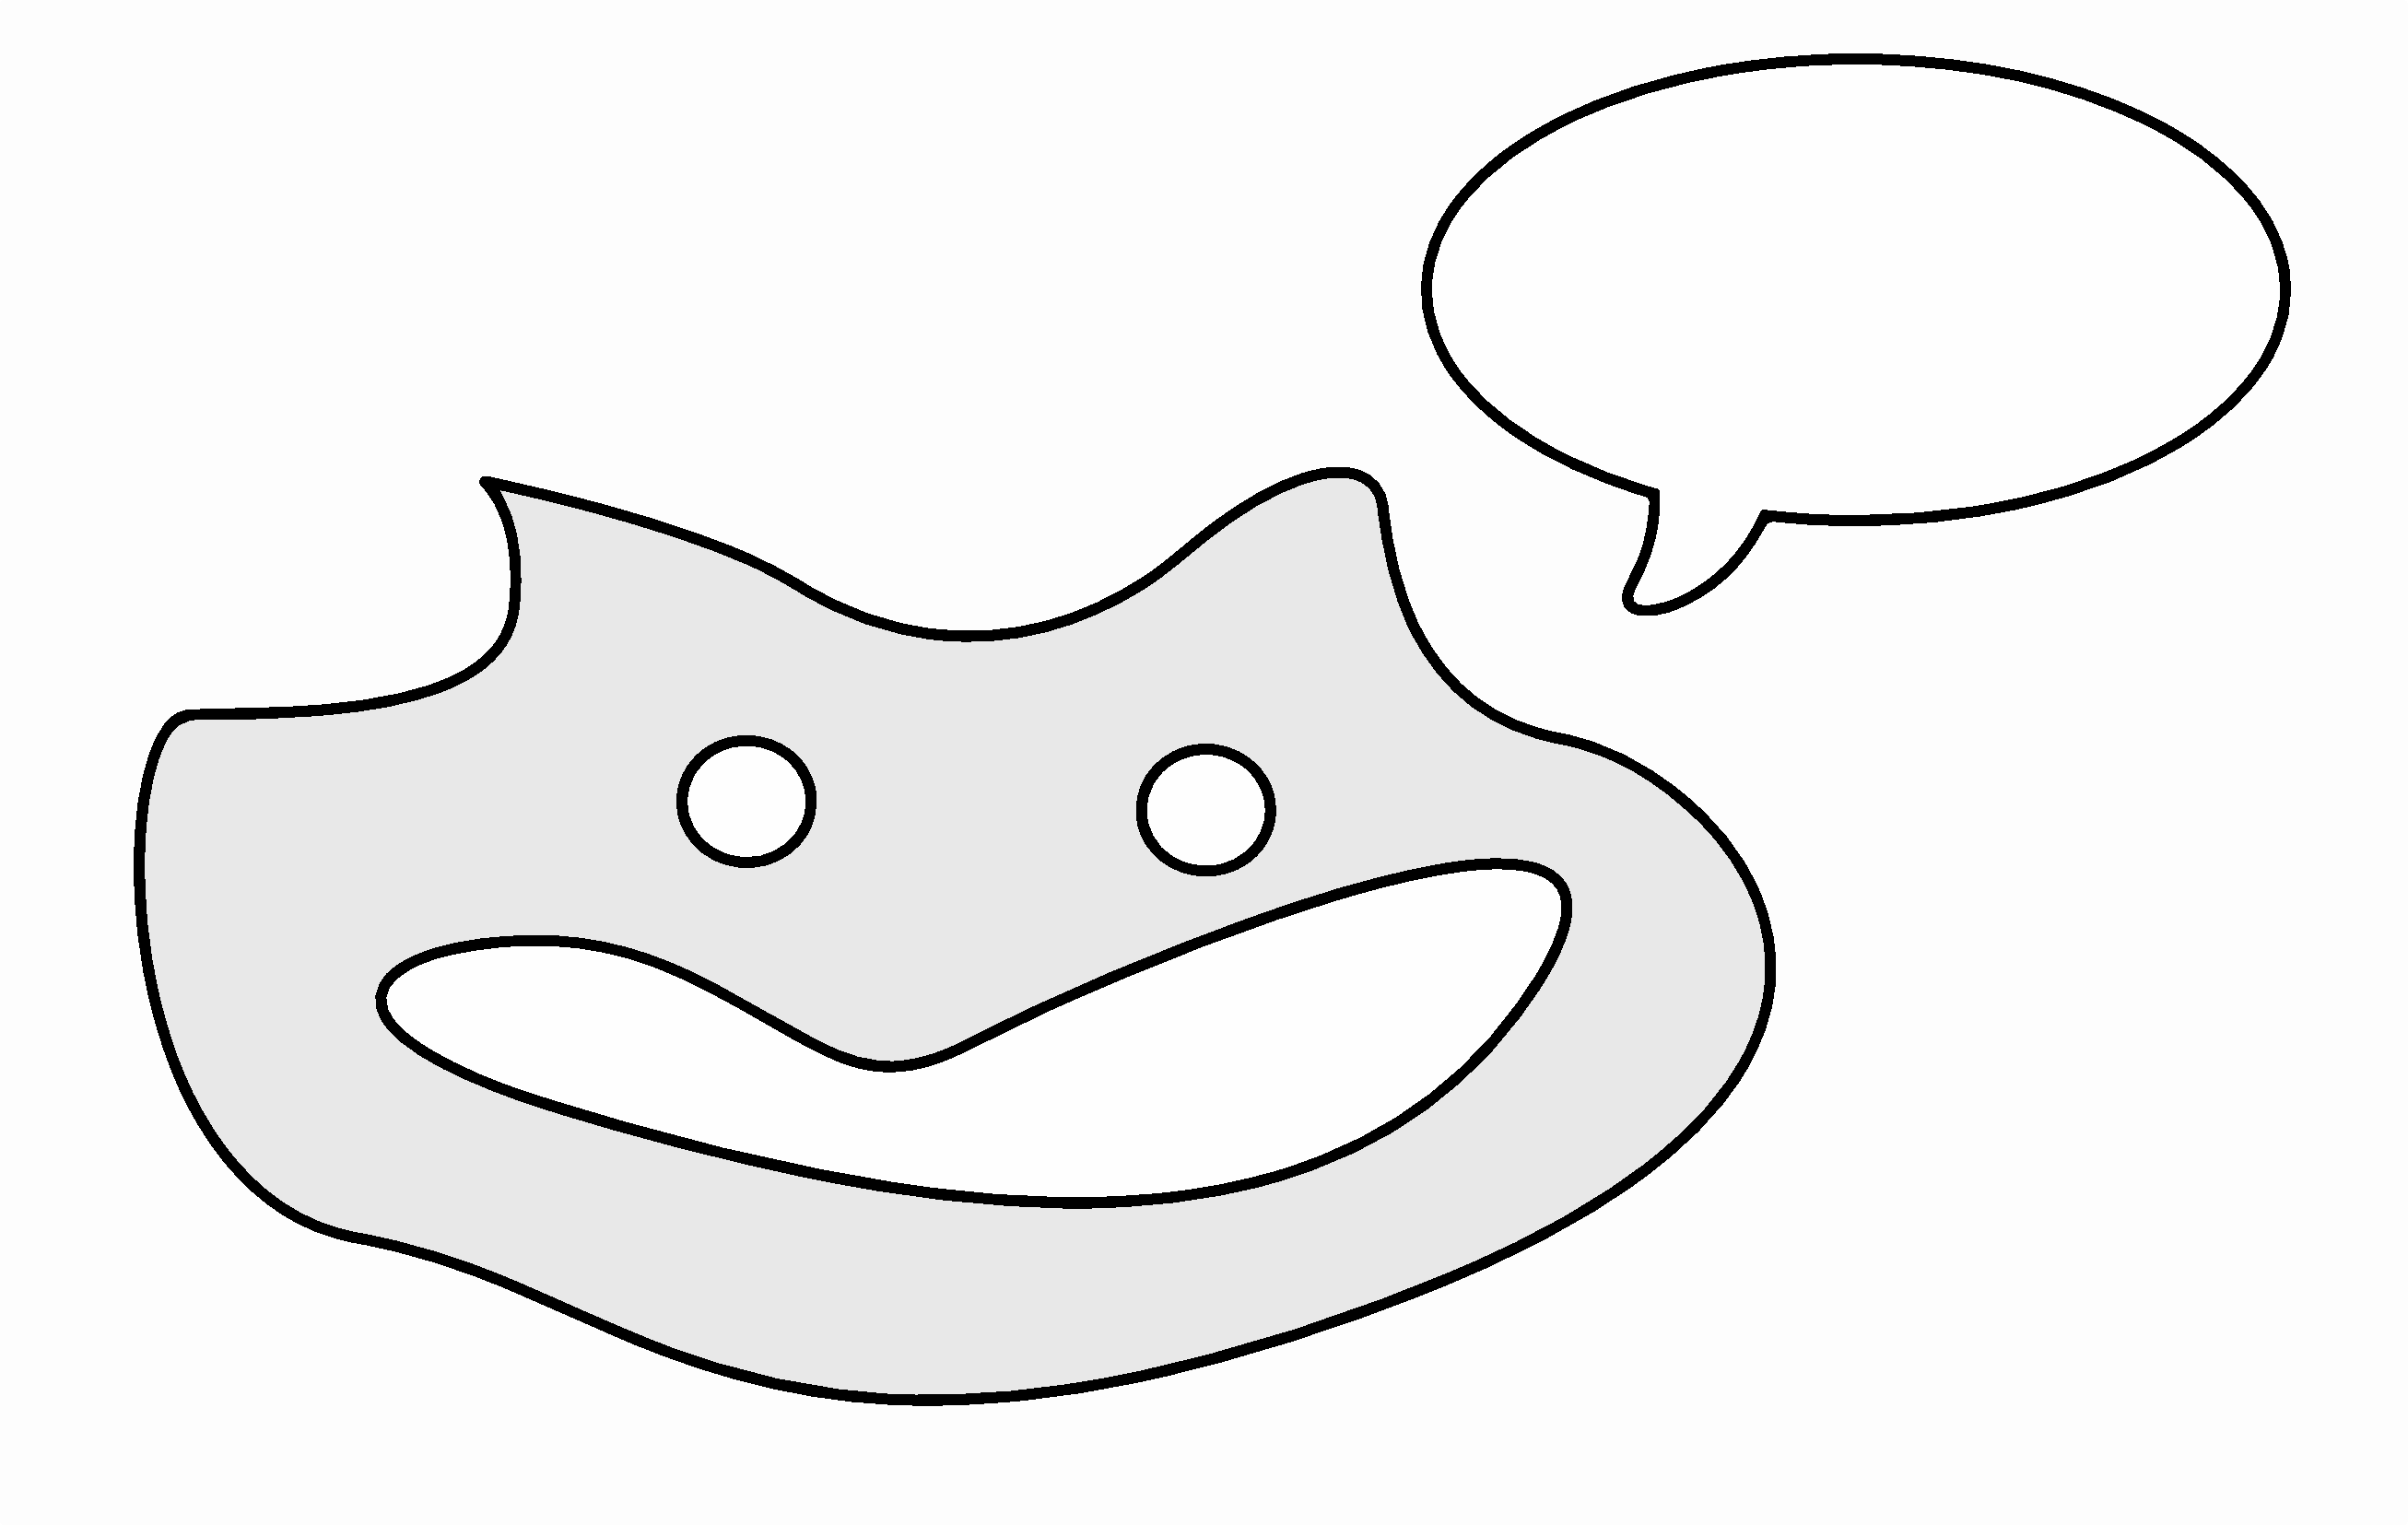
\includegraphics[width=.8\textwidth]{mu.pdf}\raisebox{30.5ex}{\makebox[0pt]{\kern-28ex\Huge\href{https://www.youtube.com/shorts/s9C03DiBU1A}{$\boldsymbol\mu $}}}}
    \end{center}
    \vskip-\medskipamount
    虽然理论上我们用 $m$ 来代表测度更为合适, 但 $m$ 这个记号在 Lebesgue 1902 年的划时代博士论文 \textit{Intégrale, longueur, aire.} 中使用了. 为了纪念他大家以后都会用 $m$ 来表示 Lebesgue 测度.
\end{alterendnote}
\begin{alterendnote}
    S. Banach 本人在此之前得到 $\mathbb R^2$ 和 $\mathbb R$ 并不会产生这种现象: 也即是在 $\mathbb R$, $\mathbb R^2$ 上存在有限可加测度, 且保持平移(旋转)不变性. 但现在观之, 此只能作为一些特例.
\end{alterendnote}
\begin{alterendnote}
    比如``一个半径为 $1$ 的三维球可分成五块并重组成两颗半径为 $1$ 的三维球''. 至于为什么是三维球, 一个有趣的科普可以见 \url{https://www.bilibili.com/video/av2674104/}.
\end{alterendnote}
\begin{alterendnote}
    或者是``物理''.
\end{alterendnote}
\begin{alterendnote}
    你可能会问为什么不用``不可数可加性'', 原因很简单, 因为我们实在是不好处理不可数个数的加法: 在后面我们处理对计数测度的积分(或者用一点点点点拓扑的知识, 用网来将序列极限推广)我们可以一瞥此类求和, 但此与可数情形无异: 求和收敛当且仅当不可数个元素中非零元至多可数, 且该可数求和绝对收敛. 同时, 可数可加性是蕴含有限可加性的, 只需令除了有限个集合外的其他集合为空集即可.
\end{alterendnote}
\begin{alterendnote}
    事实上在第二款中令 $A_n=\varnothing$, 则有``$\mu (\varnothing)=\infty\varnothing \implies \mu (\varnothing)=0$ 或 $\mu (\varnothing)=\infty$.''
\end{alterendnote}
\begin{alterendnote}
    事实上大家都承认.
\end{alterendnote}
\begin{alterendnote}
    为什么是 $\sigma $? 事实上, $\sigma $(或S) 代表德语中的 Summe(求和), 或者对集合的求和(并), 而反之 $\delta $(或D) 来自德语 Durchschnitt(交). 更一般地, 我们用``$\sigma $-''表示可数求和, 比如拓扑空间 $X$ 若是可数个紧集之并, 则称其是\;$\sigma$-紧的.
\end{alterendnote}
\begin{alterendnote}
    当然还有定义在其他结构上的测度, 不过\;$\sigma $-代数是最容易处理的.
\end{alterendnote}
\begin{alterendnote}
    有的书将其称作``可测空间'', 不过这个称呼看上去有点误导性.
\end{alterendnote}
\begin{alterendnote}
    这个定义也不是构造性的, 事实上关于一个子集生成的\;$\sigma $-代数的确有生成公式, 但是并不直观也不好处理. 一个用处是来判断\;$\sigma $-代数的势: 如果 $A$ 到 $\mathbb R$ 有一个单射, 那么 $\mathcal M(A)$ 亦然.
\end{alterendnote}
\begin{alterendnote}
    这类\;$\sigma $-代数的有特殊的作用: 比如说 $X$, $Y$ 是拓扑空间, $f:X\to Y$ 是同胚, 那么我们清楚 $f$ 诱导了 $X$, $Y$ 开集间的一一对应. 同时也诱导了 $\mathcal B_X$, $\mathcal B_Y$ 中集合(称为 Borel 集)的一一对应. 或者, 因为神说``\emph{开集要是可测的}''. 于是就有了 Borel\;$\sigma $-代数. 另外地, 由于还有 Baire $\sigma $-代数, 因此我们有时会记 Borel $\sigma $-代数为 $\mathcal{B}_{\mathrm{orel}}(X)$.
\end{alterendnote}
\begin{alterendnote}
    事实上这种东西叫做拓扑基(或者拓扑子基).
\end{alterendnote}
\begin{alterendnote}
    可数性要求是为了防止我们超出\;$\sigma $-代数只能处理可数交并补的权限.
\end{alterendnote}
\begin{alterendnote}
    一个例子是正项级数求和:对有限个正数求和我们自然可以交换求和顺序, 但对可数个呢? 通过基本的分析学我们知道这也是可以交换的, 即使得到的结果是无穷. 除此之外, 我们还关心非负可积函数列 $\{f_n\}_{n\geqslant 0}$ 会不会有\[\lim_{N \to \infty} \int \sum_{n=0}^N f_n = \int\sum_{n\geqslant 0}f_n.\](即使结果是无穷亦成立, 这看起来有点像二重求和, 虽然我们并不知道 $\sum_{n\geqslant 0} f_n$ 可积性如何), 这其实就是在之后的``单调收敛定理''. 在这种情形下, 将目标分为可数个有限的玩意, 然后分别处理之后加起来也许会有点作用.
\end{alterendnote}
\begin{alterendnote}
    这样看来,\;$\sigma $-有限测度应该叫``半有限测度''更为合适, 但不巧的是半有限测度已经有定义了:若 $E\in\mathcal M$ 且 $\mu (E)=\infty$, 则 $\exists F\subseteq E$, $\infty>\mu (F)>0$. 我们这里不会讨论这种测度.
\end{alterendnote}
\begin{alterendnote}
    如果我们考虑 Dedekind 构造实数的方式, 会发现一个数集的上确界恰好是其对应分划之并.
\end{alterendnote}
\begin{alterendnote}
    如果是拓扑的话, 只考虑序列对应的``连续性''是片面的, 但由于\;$\sigma $-代数只能处理可数次交, 并, 因此考虑序列才能变得自然.
\end{alterendnote}
\begin{alterendnote}
    这个例子来自 Giuseppe Vitali.
\end{alterendnote}
\begin{alterendnote}
    只是一种直观描述而已, 并不是对真正的圆作测度, 在套测度函数之前先把圆拉成线段吧!
\end{alterendnote}
\begin{alterendnote}
    到这里其实就需要用到选择公理.
\end{alterendnote}
\begin{alterendnote}
    事实上 Lebesgue 测度性质比较好, 其零测集的子集必然可测. 这个性质被称为``完备性'', 我们将在\hyperref[外测度与测度的完备化]{第五节}中涉及.
\end{alterendnote}
% \begin{alterendnote}
%     一个造成其繁琐的原因是我们总有办法让这个零测集子集某种意义上``可测'', 见后文测度完备化的内容.
% \end{alterendnote}
\begin{alterendnote}
    事实上, 我们对性质良好的集合可以证明 $\operatorname{inn}\operatorname{area}$, $\operatorname{out}\operatorname{cont}$ 与其的关系: 若 $A$ 是 $\mathbb R^n$ 中的开集, 则 $\operatorname{inn}\operatorname{area}A=A$; 若 $A$ 是 $\mathbb R^n$ 中的紧集, 则 $\operatorname{out}\operatorname{area}A=A$.
\end{alterendnote}
\begin{alterendnote}
    所以它才叫``容度''而不是测度.
\end{alterendnote}
\begin{alterendnote}
    这个例子其实说明 \[D(x)=
        \begin{cases}
            1, & x\in\mathbb Q,    \\
            0, & x\notin\mathbb Q.
        \end{cases}\] 的 Riemann 积分是不存在的.
\end{alterendnote}
\begin{alterendnote}
    和历史的进程一样, Harnack 考虑的``外测度''一开始也只是处理 $\mathbb R$ 上的情形, 我们在这里暂时先不管不单纯的 $\mathbb R^n$, 只处理 $\mathbb R$ 上的情形.
\end{alterendnote}
\begin{alterendnote}
    这里的 $(b_j-a_j)$ 也能换成 $F(b_j)-F(a_j)$, 其中 $F$ 是一个右连续单增函数, 我们管它叫``分布''. 比如令 $F=(\mathord{\arctan} + \pi /2)/2\pi $, 则 $F$ 是一个概率分布. 对于一般的 $F$, 我们管这样子定义的测度(在延拓之后)叫 Lebesgue\,--\,Stieltjes 测度, 直观上来看, 就相当于把 $\mathbb R$ 拉长缩短变形, 而在每点变形(缩涨)的程度刚好是 $F$ 的导数(事实上, $F$ 是几乎处处有导数的, 也就是 $F$ 不可导的点组成一个 Lebesgue 零测集).
\end{alterendnote}
\begin{alterendnote}
    这里考虑 $(a_j,b_j\,]$ 而不是看起来更简单的 $(a_j,b_j)$ 其实是因为 $(a_j,b_j\,]\cup (b_j,c_j\,]  = (a_j,c_j\,]$ 是一个新的半开半闭区间. 而不是像 $(a_j,b_j)\cup (b_j,c_j)$ 这样的中间差了一个点的东西. 事实上如果要考虑在这种中间差了一个点的东西上定义对函数 $F$ 的 Lebesgue\,--\,Stieltjes 测度的话, 势必对 $F$ 的连续性有更高的要求, 这反而是一种束缚.
\end{alterendnote}
\begin{alterendnote}
    为了令 $E\subseteq\bigcup_{j\geqslant 0}A_j$ 的 $A_j$ 选择存在, 我们不妨令 $X\in\mathscr A$.
\end{alterendnote}
\begin{alterendnote}
    除了我们将要探讨的 Lebesgue 测度, 另一个著名的外测度例子是 $\mathbb R^n$ 上的 Hausdorff 测度($\operatorname{diam}$ 是球的直径):\[
        \mathcal H^s_\delta(E)=\inf\Bigl\{ \,\sum_{j\geqslant 0}(\operatorname{diam}C_j)^s\Bigm| C_j\textit{ 是直径不大于 $\delta $ 的球体},\, E\subseteq\bigcup_{j\geqslant 0}C_k\, \Bigr\}.\]这个测度和分形维数相关, 或者我们可以称为``$s$ 维对应的\;$\delta $-外测度''. 一个例子是 Cantor 集 $C$, 令
    \[
        \mathcal H^s(C) = \lim_{\delta \to 0^+}\mathcal H^s_\delta(C).
    \]
    是 $C$ 对应的 $s$ 维 Hausdorff 外测度. 可以证明 $\exists t>0$,
    \[
        \mathcal H^s(C) = \begin{cases}
            \infty, & s<t, \\
            0,      & s>t.
        \end{cases}
    \]
    我们称 $t$ 为 Cantor 集的 Hausdorff 维数, 可以计算得到 $t = \log 2/\log 3$. 其直观描述大概是:
    \begin{itemize}
        \item 我们用低维的方法去度量高维的集合得到的结果自然是 $\infty$, 用高维的方法度量低维的集合得到的结果自然是 $0$, 对于 Cantor 集这种``有限的集合'', 应该存在一个对应的维度使得其对应度量结果是有限正数.
        \item 注意到我们将 Cantor 集的``直径''缩小为原来的 $1/3$ 得到小 Cantor 集, 两个小 Cantor 集可以拼成一个 Cantor 集. 这个事实有点违反直觉: 缩小为原来的 $1/3$ 得到小 Cantor 集应该要用 $3$ 个才可以拼成原 Cantor 集. 二维平面上的开集``直径''缩小为原来的 $k$ 倍, 则需 $1/k^2$ 个才能拼成原来的开集. ``$^2$''乃是二维所致, 因此类比一下, Cantor 集的对应维数是 $\log _32$. 我们可以将这一过程推广到其他具有严格自相似性质的集合.
    \end{itemize}
    马后炮地说, 我们只是稍稍改了下面积的定义, 在 $s$ 扫过 $[\,0,\infty)$ 的过程中总有一个令其对应测度为有限正数(Hausdorff 维数), 而这个数的大小(当然受限于底空间的维度)可以判别所讨论集合的自相似程度与粗糙性. 更多有趣的内容见 \cite{falconer86}.
\end{alterendnote}
\begin{alterendnote}
    Lebesgue 本人也给出了针对 Lebesgue 测度的可测性条件, 但和 Carathéodory 给出的不同. 事实上 Lebesgue 给出的条件非常依赖于测度的\;$\sigma $-有限性.
\end{alterendnote}
\begin{alterendnote}
    $B$ 当然可以是空集, 故 $\mathcal M\subseteq\overline{\mathcal M}$, 我们在这里跳过这个新结构是\;$\sigma $-代数的证明.
\end{alterendnote}
\begin{alterendnote}
    事实上也只能这样, 按照我们的理解, 零测集的子集必然零测, 故不应该通过并集影响测度.
\end{alterendnote}
\begin{alterendnote}
    事实上单独讨论 $\mathcal B_{\mathbb R}$ 上的测度(Borel 测度) $\mu $ 也会有不少有趣的结果. 在限制测度的有限性的前提下(比如说任意紧集的测度都有限)我们可以给出一个分布:\[F_\mu(x) = \begin{cases}
            -\mu ((x,0\,]), & x<0, \\
            0,              & x=0, \\
            \mu ((0,x\,]),  & x>0.
        \end{cases}\]同时分布可以决定一个 Lebesgue\,--\,Stieltjes 测度.
    \[\mu^F (E)=\inf\Bigl\{ \,\sum_{j\geqslant 0}\bigl(F(b_j)-F(a_j)\bigr)\Bigm| E\subseteq\bigcup_{j\geqslant 0}(a_j,b_j\,]\, \Bigr\}.\]
    而此种情况下事实上有 $\mu ^{F_\mu}=\mu $.

    考虑看起来(相比 Lebesgue 测度)不完备的 Borel\;$\sigma $-代数上的测度上的的一个重要性是很多特殊的测度的可测集都包含 $\mathcal B_{\mathbb R}$(毕竟是开集生成的\;$\sigma $-代数), 比如 Lebesgue\,--\,Stieltjes 测度. 而很多与 Lebesgue 测度相关的性质可以同样下放到一般的 Lebesgue\,--\,Stieltjes 测度上. 比如:\[\begin{aligned}
            \mu (E) & =\inf\bigl\{\, \mu (A)\bigm| E\subseteq A,\,A\textit{ 是 $\mathbb R$ 中的开集}\,\bigr\}   \\
                    & = \sup\bigl\{\, \mu (A)\bigm| A\subseteq E,\,A\textit{ 是 $\mathbb R$ 中的紧集}\,\bigr\}.
        \end{aligned}\]
    另外一个有趣例子是 $\lim_{h \to 0} (\mu / m)((x,x+h\,]) = \lim_{h \to 0} (F(x+h)-F(h))/h$ 对应的是 $F$ 的导数(当然对于这样的 $F$ 我们可以要求其不是单增的, 此时就需要考虑符号测度或者复测度). 至于真正处理此类两个测度之比值大概会在 Euclid 空间微分定理相关内容中涉及, 一个经典的例子是: 单调(或有界变差的)函数必然是几乎处处可导的------其隐晦地告诉我们可以将``沿曲线积分''的曲线从方便讨论的分段可微曲线推广成连续可求长曲线. 或者对任何一般的 Lebesgue 可积函数(关于什么是``可积''可以看后文, 事实上这里的可以也可以换成是``局部可积'', 也就是在区间 $[\,a,b\,]$ 上或紧集内可积), 我们有
    \[
        \lim_{r\to 0} \frac{1}{m(N_r(x))}\int_{N_r(x)} f = f(x),\quad N_r(x) = \{\,y\mid |y-x|<r\,\}
        .\]
    对几乎处处的 $x$ 成立. 证明这个定理需要用到Radon\,--\,Nikodym定理和一些极大函数的有界性处理(主要是从好的函数推广到一般的局部可积函数). 这样类型的定理并非特例:
    \begin{theorem}
        令$f$, $\phi$可积, 且$\phi \geqslant 0$, 径向递减(即$\exists $单减函数$\psi :[\,0,\infty)\to [\,0,\infty)$满足$\phi (x)=\psi (|x|)$), 则
        \[\lim_{t \to 0} \frac{1}{t^n}\int_{\mathbb R^n}\phi \Bigl(\frac{y}{t}\Bigr)f(x-y)\d x= \biggl(\int \phi\biggr)f(x).\]
        几乎处处的 $x$ 成立.
    \end{theorem}
    \begin{theorem}[L. Carleson, 1965]
        令$f$以$1$为周期, $\int_0^1|f|^2<\infty$, 则
        \[\lim_{N \to \infty} \sum_{n=-N}^N \hat f(n)\mathrm{e} ^{2\pi\mathrm{i}n x}=f(x).\]
        对几乎处处的 $x$ 成立. 其中$\hat f$是$f$的Fourier系数: $\hat f(n)=\int_0^{1}f(x)\mathrm{e} ^{-2\pi\mathrm{i} n x}\d x$.
    \end{theorem}
    证明的主要方法都是从性质良好的函数开始(比如光滑紧支函数或者速降函数), 然后(由光滑紧支函数或速降函数在可积函数空间内稠密)推广到可积函数空间, 其关键步骤是证明极大算子$\sup_{t > 0} |\int_{\mathbb R^n}\phi (y / t)f(x -y)/ t^n\d y |$或$\sup_{N \geqslant  0} |\sum_{n=-N}^N \hat f(n)\mathrm{e} ^{2\pi\mathrm{i}n x}|$的某种有界性, 从而从稠密集推广到整个度量空间(回想一下, 在稠密集上的一致连续函数可以唯一延拓到整个完备度量空间, 极大函数的有界性自然可以强烈地限制原算子的有界性, 而赋范线性空间间的线性映射有界和连续等价). 更多内容可以参考\cite{2001fourier}, 和\cite{miao2018}.
\end{alterendnote}
\begin{alterendnote}
    有趣的是这件事并非那么显然, 但的确是从开区间上的性质决定了 $\mathcal L$ 中集合的性质, 这需要用到 Carathéodory 延拓定理, 大概描述的是在描述一个集合(事实上应该是代数)上的测度 $\mu $ 延拓到该集合生成的\;$\sigma $-代数上的测度 $\mu_{\sigma } $ 在 $\mu $ 是\;$\sigma $-有限的前提下, 延拓是唯一的. 故生成的\;$\sigma $-代数可由代数上的测度直接决定. 当然也可以依靠外测度的定义直接证明.
\end{alterendnote}
\begin{alterendnote}
    正所谓``\textit{任何同函数论有关的问题都将导致同集合论有关的某些问题, 只要后面这种问题获得解决或者可能解决, 原有问题就可以随之解决或者近乎解决}.''~------René Baire
\end{alterendnote}
\begin{alterendnote}
    事实上这个记号也有其他意义: $\int_\varnothing \infty$ 应当是 $0$. 但 $\varnothing$ 只是作为最平凡的零测集的例子, 我们想把这个想法延拓到其他零测集上面.
\end{alterendnote}
\begin{alterendnote}
    我们这里不会称为``可积的'', 因为这些函数的积分可能是 $\infty$, 而此种情况我们不会认为函数``可积''.
\end{alterendnote}
% \begin{alterendnote}
%     一个最朴素, 直观的差距是测度上的积分对应了比Riemann积分更强的分解: 若$X=\bigcup_{\alpha \in A}U_ \alpha $, 则$f=\sum_{\alpha \in A}f\chi_{U_ \alpha }$. 直接类比Riemann积分: 其对应的是$U_ \alpha$是子区间的情形, 应此受制于连续性; 而测度上的积分只需$U_ \alpha $可测, 某种意义上会比Riemann积分更广阔些.
% \end{alterendnote}
\begin{alterendnote}
    事实上我们关注的主要是函数列的上 / 下极限, 上 / 下确界, 因为按我们以前关于\;$\sigma $-代数和测度的处理, 我们只能处理可数个对象.
\end{alterendnote}
\begin{alterendnote}
    我们在这里不写\[\left| \int \psi _n\d \mu-\!\int f\d \mu  \right|\to 0. \]是为了防止 $\infty-\infty$ 的情形.
\end{alterendnote}
\begin{alterendnote}
    自然, 此处用半开半闭区间是为了让我们的分割能首尾相连: 如果用开区间则端点不会被考虑, 用闭区间端点会重复考虑.
\end{alterendnote}
\begin{alterendnote}
    事实上, 与 $f^{-1}([\,a,b\,])$, $f^{-1}((a,b))$, $f^{-1}((a,\infty\,])$, $f^{-1}([\,-\infty,a))$ 可测都等价.
\end{alterendnote}
\begin{alterendnote}
    你可能会想要知道 $\overline{\mathbb R}$ 上的开集是什么, 毕竟是由他们生成了 $\mathcal B_{\overline{\mathbb R}}$. 事实上 $\overline{\mathbb R}$ 就是 $\mathbb R$ 中的开集或者 $\mathbb R$ 中的开集并上 $[\,-\infty,a)$ 或 $(a,\infty\,]$. 一个另一个直观的想法是将 $\overline{\mathbb R}$ 视为是 $[\,0,1\,]$ (比如说复合 $ (\mathord{\arctan} + \pi /2 ) /\pi $), 然后 $[\,0,1\,]$ 上的开集视为 $A\cup [\,0,1\,]$, 其中 $A$ 是 $\mathbb R$ 中的开集.
\end{alterendnote}
\begin{alterendnote}
    如果你要考虑打到 $\mathbb R^n$ 之类的可测函数, 那么定义会稍稍复杂些. 我们此处不处理这些函数.
\end{alterendnote}
\begin{alterendnote}
    另一个暂时性的诠释是, (若读者知晓拓扑的定义的话) $\sigma $-代数和拓扑在某种意义上有些相似: 拓扑应当对有限交与任意并封闭, 而\;$\sigma$-代数对可数交和可数并(以及补)封闭. 事实上, 两个拓扑空间 $(X,\mathcal T)$, $(Y,\mathcal P)$ 间的连续映射 $f:X\to Y$ 应满足\[\forall G\in \mathcal P,\quad f^{-1} (G)\in\mathcal T.\]此与可测空间间的可测函数相对应\[f:(X,\mathcal M_1)\to (Y,\mathcal M_2),\quad \forall A\in\mathcal M_2,\quad f^{-1} (A)\in\mathcal M_1.\]因此广泛点说, 可测函数是保持两个可测空间的\;$\sigma $-代数上结构的映射, 或者称为可测空间组成的范畴之态射, 如同连续映射对拓扑空间, 全纯函数对复空间一般.

    另外地, 看上去\;$\sigma $-代数像是在拓扑的定义上稍作修改, 而我们自然关心这种修改会让其各自对应的``保持结构的映射''改变多少, 也即连续映射与可测映射的关系. 一个著名的定理是 Luzin 定理:
    \begin{theorem}[Luzin]
        对于 $[\,a,b\,]$ 上的可测函数 $f$, 对任意 $\varepsilon>0$, $\exists E_\varepsilon\subset[\,a,b\,]$ 且 $m(E_\varepsilon)<\varepsilon$, $f$ 在 $[\,a,b\,]\setminus E_\varepsilon$ 上连续.
    \end{theorem}
    大概就是我们对拓扑定义的修改所得到对应映射的差异可以被测度控制. 其次, 拓扑中亦有生成的概念:
    \[
        \mathcal T(A) = \textit{包含 $A$ 的最小拓扑} = \bigcap_{T,\textit{拓扑}\atop A\subset T}T,\quad A\subset\mathcal P(X)
        .\]
    不过拓扑的生成与\;$\sigma $-代数的生成有相当大的区别: 最大的区别来自拓扑只要求有限交封闭, 因此我可以让 $A$ 中元素任意有限交得到``原子集合'', 再自由地并起来即可. 因此, 对于拓扑的生成我们有简明的公式
    \[
        \mathcal S(A) = \biggl\{~ G \;\biggm|\; G = \bigcap_{U\in B\atop \mkern-8mu B\subset A,\textit{有限子集}\mkern-8mu} U ~\biggr\},\quad \mathcal T(A) = \biggl\{~ H \;\biggm|\; H = \bigcup_{G\in B\atop B\subset \mathcal S(A)} G ~\biggr\}
        .\]
    或者
    \[
        \mathcal T(A) = \biggl\{~\bigcup_{\textit{任意}}\bigcap_{\textit{有限}} G\;\biggm|\; G\in A  ~\biggr\}
        .\]
    而\;$\sigma $-代数的生成公式则要复杂许多.

    最后一个例子是乘积\;$\sigma $-代数: $\{\mathcal M_ \alpha\}_{\alpha\in A}$ 是\;$\sigma $-代数族, 则乘积\;$\sigma $-代数规定为 $\prod_{\alpha\in A}X_\alpha$ 上令投影映射 $\pi_\alpha$ 可测的最小\;$\sigma $-代数 $\bigotimes_{\alpha\in A}\mathcal M_\alpha$. 因为在前面说过, $\pi_\alpha$ 作为标准的投影映射必然是要保持\;$\sigma $-代数上结构才行, 也即是可测, 而最小\;$\sigma $-代数是因为最大\;$\sigma $-代数 $\mathcal P(\prod_{\alpha\in A}X_\alpha)$ 是平凡的. 一言蔽之:
    \[
        \begin{aligned}
            \pi_\alpha \textit{ 可测} & \implies E_\alpha\in\mathcal M_\alpha, \quad\pi _\alpha^{-1} (E_\alpha) \in \bigotimes_{\alpha\in A}\mathcal M_\alpha                                               \\
                                      & \implies \bigotimes_{\alpha\in A}\mathcal M_\alpha = \mathcal M( \{\, \pi _\alpha^{-1} (E_\alpha) \mid E_\alpha\in \mathcal M_\alpha,\,\forall \alpha\in A\, \}  ).
        \end{aligned}
    \]
    而此与乘积拓扑 $\mathcal T (\{\,\bigcap_{\alpha\in B\atop B\subset A,\textit{有限子集}\mkern-8mu} \pi _\alpha^{-1} (E_\alpha) \mid E_\alpha~\textit{是}~X_\alpha \textit{ 中开集}\,\})$ 的构造不谋而合. 乘积\;$\sigma $-代数的一个作用是讨论 $\mathbb R^n$ 中的 Lebesgue 可测集, 事实上 $\mathcal L^n = \overline{\prod_{j=1}^n\mathcal L}$. 也即是在 $\mathbb R$ 的 Lebesgue 可测集乘积 $n$ 次后的完备化, 至于其对应的 Lebesgue 测度, 可由在矩形上的处理 $m^n(\prod_{j=1}^n (a_j,b_j\,]) = \prod_{j=1}^n(b_j-a_j)$ 延拓至 $\overline{\prod_{j=1}^n\mathcal L}$ 得到(事实上我们当然可以一步到位直接延拓到最大的那个\;$\sigma $-代数, 但考虑乘积拓扑可以通过完备化的方式让我们对可测集的构造有更深的理解, 因此\hyperref[AcupN]{正规性}对 $\mathbb R^n$ 中的 Lebesgue 测度也是成立的).

    至于为什么说这个诠释是暂时性的, 事实上我们可以在远弱于\;$\sigma $-代数的结构上定义测度(比如半环), 而这些结构其实与拓扑差距甚大, 因此与拓扑的类比作为引入用的暂时性例子是更合适的.
\end{alterendnote}
\begin{alterendnote}
    这里的 $L$ 其实是为了纪念 Lebesgue, 即使我们并没有处理 Lebesgue 测度.
\end{alterendnote}
\begin{alterendnote}
    其实对广义的 Riemann 积分非也, 考虑 $f(x)=\sin x /x$, 则其在 $(0,\infty)$ 上的 Lebesgue 积分不存在, 而广义黎曼积分为 $\pi /2$. 所以在某种意义上, 不绝对可积的函数就是不可积函数.
\end{alterendnote}
\begin{alterendnote}
    回忆一下我们断言对测度的积分可以将各式各样的求和统一在一起, 我们不妨用计数测度的语言来说明一下单调收敛定理和控制收敛定理:
    \begin{theorem}[单调收敛定理]
        令 $\{a_{nm}\}_{n,m\geqslant 0}$ 是正项序列, 则
        \[
            \sum_{n\geqslant 0}\sum_{m\geqslant 0}a_{nm} = \sum_{m\geqslant 0}\sum_{n\geqslant 0}a_{nm}
            .\]
        允许求和值为 $\infty$ 的情形.
    \end{theorem}
    \begin{theorem}[控制收敛定理]
        令 $\{a_{nm}\}_{n,m\geqslant 0}$ 是复数序列, 且满足 $\lim_{n \to \infty} a_{nm} = A_m$. 若
        \[
            \sum_{m\geqslant 0}\Bigl(\sup_{n\geqslant 0} |a_{nm}|\Bigr) <\infty
            .\]
        则
        \[
            \lim_{n \to \infty}\sum_{m\geqslant 0}a_{nm} = \sum_{m\geqslant 0}A_m < \infty
            .\]
    \end{theorem}
\end{alterendnote}
\begin{alterendnote}
    事实上, Riemann 积分中也有相似的控制收敛定理:
    \begin{theorem}
        $\{f_n\}_{n\geqslant 0}$ 是定义在 $[\,0,\infty)$ 上的函数列, 且在 $\forall[\,a,b\,]\subseteq[\,0,\infty)$ 上 Riemann 可积, 且 $f_n\to f$, 其中 $f$ 在 $\forall[\,a,b\,]\subseteq[\,0,\infty)$ Riemann 可积, 若存在 Riemann 可积函数 $g$ 满足 $|f_n|\leqslant g$ 对任意 $n$ 成立, 且 $\int_{[0,\infty)}g<\infty$, 则  \[\lim_{n \to \infty} \int_{[0,\infty)} f_n = \int_{[0,\infty)} f.\]
    \end{theorem}
    \noindent 有关这个定理的细节可以参考\cite{Cunningham67} (事实上这个定理也可以通过 Lebesgue 测度下的控制收敛定理马后炮地推出来).
\end{alterendnote}
\begin{alterendnote}
    也就是\[\nu (E)=\inf\Bigl\{ \,\sum_{j\geqslant 0}\bigl(F(a_j)-F(b_j)\bigr)\Bigm| E\subseteq\bigcup_{j\geqslant 0}(a_j,b_j\,]\, \Bigr\}\]其中 $F$ 是单增右连续函数.
\end{alterendnote}
\begin{alterendnote}
    事实上, 这样的 $f$ 并不是唯一的, $f$ 自然可以在一个\;$\mu $-零测集下乱跑, 只需保证是可测的即可. 同时, 由于 $\nu $ 和 $\mu $ 都是非负的, 因此 $f$ 也是几乎处处非负的, 若要考虑 $\mathbb R$ 甚至 $\mathbb C$ 上的函数, 则须引入符号测度或复测度.
\end{alterendnote}
\begin{alterendnote}
    事实上, Radon\,--\,Nikodym 定理阐明, 如果 $\nu$ 对 $\mu $ 绝对连续, 其中 $\nu$ 可以是一般的(正)测度, 也可以是符号测度或者复测度, $\mu $ 是正测度, 且两个测度都是\;$\sigma $-有限的, 且定义在同一个\;$\sigma $-代数上. 那么满足
    \[
        \nu (E) = \int_E f\d \mu
        .\]
    的 $f$ 必然存在, 且在相差一个\;$\mu $-零测集的情形下唯一.
\end{alterendnote}
\begin{alterendnote}
    事实上这个奇特的``测度的绝对连续''定义与函数的绝对连续之间有强烈的关联: 对于一个右连续有界变差函数 $F$(且满足 $\lim_{x\to -\infty}F(x) = 0$), 其生成的 Lebesgue\,--\,Stieltjes 测度 $\mu ^F$ 对 Lebesgue 测度绝对连续当且仅当 $F$ 在 $\mathbb R$ 上绝对连续. 至于什么是有界变差, 其实我们考虑一个(可以是不单调的)右连续函数生成的 Lebesgue\,--\,Stieltjes 测度. 我们(自然)希望有
    \[
        \begin{aligned}
            \mu ^F((a,b\,]) & = \sum_{n\geqslant 0}\mu ^F((x_n,x_{n+1}\,])                                                         \\
                            & = \sum_{n\geqslant 0}(F(x_{n+1})-F(x_n)),    & \quad a=x_0<x_1<x_2\cdots <\lim_{n \to \infty} x_n=b. \\
        \end{aligned}
    \]
    是绝对收敛的(更好的情形是无论如何选取 $\{x_n\}_{n\geqslant 0}$, $\sum_{n\geqslant 0}|F(x_{n+1})-F(x_n)|$ 总是有一个共同上界). 因为这个求和本来就不应该与我们的求和顺序相关(由于 Riemann 重排定理, 条件收敛的级数可以通过重排收敛到任何值). 因此我们有了以下要求:
    \[
        \mathop{\vcenter{\hbox{\LARGE$\mathbf{V}$}}}_{[a,b]}F \coloneqq \sup_{n\geqslant 0}\biggl\{\,\sum_{j=0}^n|F(x_{j+1})-F(x_j)|\biggm|a=x_0<x_1<\cdots <x_n=b\,\biggr\} < \infty
        .\]
    此时称 $F$ 是 $[\,a,b\,]$ 上的有界变差函数. 另外地, 选取这个定义还与曲线的长度相关: 若 $F:[\,a,b\,]\to \mathbb C$, 则 $\mathop{\vcenter{\hbox{\Large$\mathbf{V}$}}}_{[a,b]}F$ 实际上是 $\operatorname{im}F$ 的长度.

    粗略地来说, 有界变差是对可求长曲线的推广, 也是对单调函数的推广(因为有界的单调函数必然是有界变差的, 事实上, 打到 $\mathbb R$ 上的有界变差函数可以写为两个单增函数之差). 在之前的注记中提到过, 有界变差函数几乎处处有导数, 因此对于可求长曲线, 其切向量几乎处处存在, 这让沿着可求长曲线的积分称为了可能.

    有趣的是, 有界变差的定义并非来自对测度的处理, 事实上, 有界变差要求 $F$ 在局部的振幅不应过大, 而 Fourier 级数的收敛亦与振幅直接相关. 事实上, Jordan 在 1881 年的一篇论文 \emph{Sur la série de Fourier} 中引入了这个概念.

    回到对单调函数的讨论中来. 我们可以对单调(递增)函数作以下著名的分解:
    \[f = f_{\mathrm D} + f_{\mathrm{AC}} + f_{\mathrm{SC}}.\]
    其中三者都有独特的性质:
    \begin{itemize}
        \item $f_{\mathrm D}$ 是一个``离散(Discrete)''的函数: $\sum_{n\geqslant 0}a_n\chi_{\{b_n\}}$, 其实代表着 $f$ 的不连续点, 减去这些不连续点所造成的差之后 $f$ 就连续了;
        \item $f_{\mathrm{AC}}$ 可以求导, 且满足微积分基本定理: \[\int_a^b f_{\mathrm{AC}}' = f_{\mathrm{AC}}(b)-f_{\mathrm{AC}}(a).\] 根据微积分基本定理我们知晓此时 $f_{\mathrm{AC}}$ 绝对连续(Absolutely Continuous);
        \item $f_{\mathrm{SC}}$ 比较特殊, 其对应的是``导数几乎处处为 $0$ 但是并不是常数函数''的函数. 事实上, 由 Fatou 引理我们可以得到: \[f(b) - f(a) \geqslant \int_{a}^b f'.\] 而 $f_{\mathrm{SC}}$ 就是其中 $f(b) - f(a) > \int_{a}^b f'$ 的那一部分. 此时 $f_{\mathrm{SC}}$ 是奇异连续(Singular Continuous)的. 一些不太雅观的例子就像是``严格单增但导数几乎处处为 $0$'' 的连续函数一样(见\,\cite{Brown69}).
    \end{itemize}
    由于一般的有界变差函数可以由单调函数拼成, 因此这个分解也可以对一般的有界变差函数有效, 在某种意义上这属于我们对一个有界变差函数分解的最终情形.
\end{alterendnote}
\begin{alterendnote}
    \label{Fubini}事实上, 这个结果也可以推广到一般的\;$\sigma $-有限测度. \par 说点题外话, 读者会发现我们列举的许多定理都要求\;$\sigma $-有限测度, 事实上在这些定理的经典证明中, 往往都是先对有限测度讨论, 然后再通过可数相加推广到\;$\sigma $-有限测度.\;$\sigma $-有限测度最著名的例子当然是 Lebesgue 测度, 非\;$\sigma $-有限测度的典例当属不可数集上的计数测度. 因此某种意义上, 计数测度虽然看起来简单, 但却与某些反例息息相关. 至于有限测度有什么优点\,$\mathinner{\ldotp \ldotp \ldotp\ldotp \ldotp \ldotp}$\,我想最直观的应当是对集列下降情形的连续性 \hyperref[测度的连续性:集列下降]{(点这儿!)}.
\end{alterendnote}
\begin{alterendnote}
    Fubini\,--\,Tonelli 定理看似只是处理普通的积分换序问题------很容易和多元微积分中的 Fubini 定理类比, 但正如尾注 \ref{Fubini} 所说的, Fubini\,--\,Tonelli 定理可以推广到\;$\sigma $-有限测度的情形: 比如可数集上的计数测度.
    \begin{theorem}[Fubini, Tonelli]
        令 $f$ 是测度空间 $(X,\mathcal M)$ 上的可测函数, $\mu _1$, $\dots $, $\mu _n$ 是定义在 $\mathcal M$ 上的\;$\sigma $-有限测度, 则:

        若 $f\geqslant 0$ 或 $f\in L(\mu_1 \times \cdots \times \mu _n)$, 则
        \[
            \int f \d (\mu_1\times \cdots \times \mu _n) = \int\left(\,\cdots \!\int\left(\, \int f \d \mu_1 \right) \d \mu_2\cdots \right)\d \mu_n
            .\]
    \end{theorem}
    考虑可数集上的计数测度如下:
    \begin{theorem}
        令 $\{\,f_n: \mathbb R^d\to \mathbb C\,\}_{n\geqslant 0}$ 是可测函数列, 则若 $\sum_{n\geqslant 0}\int |f_n|\d m^d<\infty$, 则
        \[
            \sum_{n\geqslant 0}\biggl(\int f_n\d m^d\biggr) = \int_{\mathbb R^n}\biggl(\,\sum_{n\geqslant 0} f_n\d m^d\biggr)
            .\]
    \end{theorem}
\end{alterendnote}
\begin{alterendnote}
    在这之中有一个看起来相当麻烦的问题: 事实上$\int f(x_1,\dots,x_n)\d x_1$可能并不是对所有的$(x_2,\dots,x_n)$都是可测的, 我们只能证明其对几乎处处的 $(x_2,\dots,x_n)$ 都可测, 因此我们必然要考虑这个函数在一个零测集上面是没有定义的. 由于是零测集(事实上还依赖于 Lebesgue 测度的完备性), 我们不妨把没有定义的地方补 $0$ 以便继续积分. 用看起来比较高级点的语言来说就是我们是对``函数的等价类''进行积分, 这些函数几乎处处有定义, 且两个函数等价当且仅当他们在定义域交集内相等.
\end{alterendnote}

\maketitle
\tableofcontents
\begin{tikzpicture}[remember picture,overlay]
    \draw[line cap=round, ->, white!10!black, thick] (zero) to (i);
    \draw[line cap=round, ->, white!20!black, thick] (i) to (ii);
    \draw[line cap=round, ->, white!30!black, thick] (ii) to (iii);
    \draw[line cap=round, ->, white!40!black, thick] (iii) to (iv);
    \draw[line cap=round, ->, white!50!black, thick] (iv) to (v);
    \draw[line cap=round, ->, white!60!black, thick] (v) to (vi);
    \draw[line cap=round, ->, white!70!black, thick] (vi) to (vii);
\end{tikzpicture}
\definecolor{DarkTurquoise}{rgb}{0, .48, .48}
\clearpage
\begin{abstract}
    这是一篇科普风格的文章. 因此对于文中所述定理, 我并不会全部给出证明\enote . 大多数具体的证明可见 \cite{Folland99}.

    这篇文章的本意是想要把一些测度的构造说清楚, 诚然, 测度的构造有许多种路径, 本文只是选取笔者最熟悉的一种路径, 同时对构造中所遇障碍以及对测度的积分进行一些阐述: 第一到第六节循序渐进地阐述了标准的实分析内容: 测度的构造, 延拓和 Lebesgue 测度; 第七节按照惯例阐述对测度的积分, 但自然而然地, 对积分的介绍不可避免地变得相当冗长, 几乎用了全文的一半内容才堪堪完成任务. 本文另一个特殊的点是注释繁多: 主要用于介绍测度相关的其余内容和一些对积分, 求导的处理, 终究是实分析的主干内容之一, 但因各种原因含量远超预算, 此主要由于笔者写作风格随性所致. 虽言``写科普要做减法'', 但笔者无法合理地处理注释的删减, 因此在此版本中保留了所有注释, 并将其置于文末以便提升正文阅读体验. 虽然, 但笔者仍然认为注释是本文中相当有趣的一部分, 笔者在此记录了不少自身的理解以及某些板块之间的联系(以及\hyperref[可爱猫猫]{可爱猫猫的图片}), 某种意义上也算是(超大量的)饭后甜品, 食之无妨.

    因笔者能力有限, 故差错难以避免, 还望读者海涵.
\end{abstract}
\setcounter{page}{1}
\section{引\kern\ccwd 论}
\begin{quote}
    少女祈祷中\,$\mathinner{\ldotp \ldotp \ldotp\ldotp \ldotp \ldotp}$
\end{quote}

测度(measure)一词可望文生义地理解为对集合``大小''之描述. 如: 从古希腊时期始, 数学家们就为了给出圆的面积做了许多工作; 而放到现在来看, 面积, 体积, 长度等描述其实都是 Lebesgue 测度上在良好性质集合下之限制. 为了避免把路走窄, 我们并不会从 Lebesgue 测度开始引入. 而是先介绍另一种``离散''的测度.

\begin{defi}[计数测度]
    令 $X$ 是集合, $\mathcal P(X)$ 是集合的子集所构成的集合, 也即``幂集''. 定义函数 $\operatorname{card}:\mathcal P(X)\to \mathbb Z_{\geqslant 0}\cup\left\{ \infty \right\}$. 返回集合中元素个数, 若集合无穷则返回 $\infty$\enote.
\end{defi}
诚然, 这是一种粗糙的测量集合的方法, 我们现在应该从中提取和一般``体积'', ``面积''之类描述相同的性质以为己用. 事实上, 我们并不会多关注这个测度, 将这个测度放在一开始的初衷在于让大家看到测度的其他潜能, 这种潜能我们会在后续的描述中逐步揭晓.
\paragraph{``测度''的性质, Ver.1}
\begin{itemize}
    \item 古老的测度是用来描述圆, 正方形这类几何对象的, 从现在的观点上看, 这些对象只是 $\mathbb R^2$ 上的良好子集, 因此不妨设有一个大空间 $X$, 而测度描述其子集返回一个正数(或者 $\infty$). 也即 $\mu\enote :\mathcal P(X)\to [\,0,\infty\,]$.
    \item 测度应该满足一定意义上的``可加性'', 直观上来看就是两个不交的几何对象的体积应该是其体积之和. 也即:
          \[
              A\cap B=\varnothing\implies \mu (A\cup B)=\mu (A)+\mu (B).
          \]
          当然这性质可以归纳到有限个两两不交集合的情形, 我们称此性质为``有限可加性''.
    \item 对于 $\mathbb R^n$ 中的测度, 还应该满足旋转, 平移不变性. 更一般地, 它也应当有合理的伸缩性质, 也即:
          若 $T$ 是 $\mathbb R^n$ 上的线性变换, 那么应当有 $\mu (T(E)) = |\!\det T|\cdot \mu (E)$. 此处我们稍稍利用了下 $\mathbb R^n$ 上线性变换的几何直观.
\end{itemize}
直觉告诉我们这个``测度''的性质, 或依赖该性质的定义是没有什么太大的意义的, 否则也不会出现在本文的开头. 问题出现在有限可加性与旋转, 平移不变性之间. 在 1924 年, S. Banach and A. Tarski 在一篇令人惊讶的论文 \emph{Sur la decomposition des ensembles de points en parties respectivement congruentes} 中证明了这样的事实:
\begin{theorem}[S. Banach, A. Tarski]
    令 $A$, $B$ 是 $\mathbb R^n$ 中的开集, 其中 $n\geqslant 3$. 则我们可以将 $A$, $B$ 分为同样多份: $A_1$, $\dots$, $A_k$, $B_1$, $\dots$, $B_k$ 且 $A_i$ 两两不交, $B_i$ 亦然. 且各 $A_i$ 可由 $B_i$ 旋转, 平移得到\enote.
\end{theorem}
这个定理一般被称为 Banach\,--\,Tarski 定理, 或者在现在网络的普及下, ``\emph{分球悖论}\enote''这个名字流传更为广泛. 证明这定理的过程需要用到一个叫做选择公理的集合论假设, 通俗来说其保证了无穷个集合的 Cartesian 积的存在性.

因此我们的有限可加``测度''幻梦在这机械降神下突然破灭. 这启迪我们, $\mathbb R^n$ 并非那么单纯. 我们需要削减测度的要求才能继续向前.

思来想去, 既然连``有限可加''那么``显然''\enote 的性质都会在选择公理的作用下毁灭, 那咱不如摆烂: 直接讨论所有``可测''的集合, 换句话说就是我无论怎么玩弄都不会产生任何悖论的集合. 而如何得到这样的集合就是一个重点.

在引入``可测集合''的概念之前, 我们仍需引入测度. 考虑到我们可能需要在一些特殊的可数集上面做文章: 比如 $\mathbb Q$ 之类, 亦或者能够对更多的集合(尤其是与可数个小集合的并相关)都保有良好的性质, 我们处理测度时会把``有限可加性''加强为``可数可加性\enote'', 也即: 若 $\{A_n\}_{n\geqslant 0}$ 两两不交, 则 \[\mu \biggl(\,\bigcup_{n\geqslant 0} A_n\biggr) = \sum_{n\geqslant 0} \mu (A_n).\]

\paragraph{``测度''的性质, Ver.2}\label{测度的性质}
\begin{itemize}
    \item $\mu :\mathcal M_\mu\to [\,0,\infty\,]$. 其中 $\mathcal M_\mu$ 是性质良好集合的集合.
    \item $\{A_n\}_{n\geqslant 0}$ 两两不交, $\mu (\bigcup_{n\geqslant 0} A_n) = \sum_{n\geqslant 0} \mu (A_n)$.
    \item 我们稍稍加上一个新的假设: $\mu (\varnothing) = 0$\enote. 因为测度函数返回的值最好不要太大.
\end{itemize}
这已经是我们现在处理的测度了, 不过我们需要知道 $\mathcal M_\mu$ 到底是什么.

\section[$\sigma $-代数]{$\boldsymbol{\sigma}$-代数}

\begin{quote}
    选择公理? 是不可能承认的, 这辈子都不可能承认的\enote!
\end{quote}



\begin{defi}[($\sigma$\enote-)代数\enote, 测度空间\enote]
    令 $X$ 是集合, $\mathcal M \subseteq \mathcal P(X)$ 若满足以下条件
    \begin{itemize}
        \item $\varnothing\in \mathcal M$;
        \item $A\in\mathcal M\implies A^\complement\in \mathcal M$;
        \item $A$, $B\in \mathcal M\implies A\cup B\in\mathcal M$.
    \end{itemize}
    我们管这样的集合称为代数, 如果还满足 $\{A_n\}_{n\geqslant 0}\subseteq\mathcal M$, $\bigcup_{n\geqslant 0} A_n\in\mathcal M$. 则我们管它叫\;$\sigma $-代数. 同时, 由于$\sigma $-代数和测度联系在一起, 我们命 $(X,\mathcal M)$ 为测度空间.
\end{defi}
由此可见, 我们的``可测集''至少得构成一个\;$\sigma $-代数, 这样才有比较丰富的讨论价值. 但问题是,\;$\sigma $-代数是不好处理的------其上面的定义并不能让我们有直观感受, 我们在此举一些例子:
\begin{description}
    \item[平凡的例子] 比如说 $\mathcal P(x)$ 本身或者 $\{\varnothing,X\}$.
    \item[可数-余可数\;$\boldsymbol\sigma $-代数] 令 $\mathcal M=\bigl\{\,A\subseteq X\bigm| A\textit{ 可数或~} A^\complement\textit{ 可数}\,\bigr\}$.
\end{description}
考虑到\;$\sigma $-代数的抽象性, 我们急需使用新的方法来表征\;$\sigma $-代数, 这个方法其实就是老生常谈的``生成''. 我们先回顾下($\mathbb F$ 上)线性空间的生成:

一组向量 $b_1,\dots,b_n$ 生成的子空间是包含 $b_1,\dots,b_n$ 的最小子空间, 而这个子空间有明确的构造:
\[
    \left<b_1,\dots,b_n \right> \coloneqq \biggl\{\, \sum_{j=1}^n x_jb_j \biggm| x_1,\dots,x_n\in\mathbb F \,\biggr\}
    .\]
因此对这个``子空间''的研究可以通过对 $b_1,\dots,b_n$ 的研究来实现. 至于对无穷个(甚至不可数个)向量 $\{b_ \alpha \}_{\alpha\in A}$ 张成的子空间, 我们并不能那么方便地构造, 而且构造方法和有限情形有不少区别, 我们唯一知道的情形是其生成的子空间是包含这无穷个向量的最小子空间, 因此我们只能定义为:
\[
    \mathop{\text{``min\kern-.1ex''}}\bigl\{\,E \textit{ 是子空间} \bigm| \forall\alpha\in A,\, b_ \alpha \in E\,\bigr\}
    .\]
为了实现这里的 $\min$, 由于子空间的任意交都是子空间. 因此所有子空间的交必然会退化到最小的那一个子空间:
\[
    \mathop{\text{``min\kern-.1ex''}}\bigl\{\,E \textit{ 是子空间} \mid \forall\alpha\in A,\,b_ \alpha \in E\,\bigr\} = \bigcap_{E,\textit{子空间}\atop \mkern-8mu\forall\alpha\in A, b_ \alpha \in E\mkern-8mu}E
    .\]
回到对\;$\sigma $-代数的处理上来, 由于\;$\sigma $-代数的任意交仍然是\;$\sigma $-代数. 因此定义由子集生成的\;$\sigma $-代数为:
\begin{defi}[$\sigma$-代数的生成]
    令 $X$ 是集合, $A\subseteq \mathcal P(X)$, 则其生成的\;$\sigma $-代数为
    \[
        \bigcap_{\mathcal M, \sigma\text{-代数}\atop A\subseteq \mathcal M}\mathcal M \eqqcolon \mathcal M(A)
        .\]
    大家都喜欢这样子表示``生成''\,\enote. 特别地, 生成元也可以某种程度上地简化: 如果存在另外一个集合 $B\subseteq A\subseteq\mathcal P(X)$, $A\subseteq\mathcal M(B)$, 由于 $B\subseteq A\implies \mathcal M(B)=\mathcal M(A)$ 和 $A\subseteq\mathcal M(B)\implies \mathcal M(A)\subseteq\mathcal M(B)$. 故 $\mathcal M(A)=\mathcal M(B)$.
\end{defi}
这样我们可以通过讨论\;$\sigma $-代数的生成元来讨论\;$\sigma $-代数, 如果这些生成元是有限(此时其生成的\;$\sigma $-代数也是有限的, 你可以认为是这有限个集合之间随意地交组成的``原子''集合的并)或者可数的, 那就更好了.

在此有一种生成\;$\sigma $-代数是特殊的:
\begin{defi}[Borel $\sigma $-代数]
    一个拓扑空间 $X$ 里面的开集族(如果你不知道什么是拓扑空间里的开集, 那就把它当成 $\mathbb R$ 中的开集) $\mathcal T\subseteq X$ 生成的\;$\sigma $-代数记为 $X$ 上的 Borel\;$\sigma $-代数, 其中元素称为 Borel 集合. 记为 $\mathcal B_X$\enote.
\end{defi}
一个特殊的 Borel 集的例子是 $\mathbb R$ 上的 Borel 集. 由于 $\mathbb R$ 上的开集都是至多可数个开区间之并, 故 $\mathbb R$ 上开集生成的\;$\sigma $-代数与开区间生成的\;$\sigma $-代数一致. 也即:
\[
    \mathcal  B_{\mathbb R} = \mathcal M\left( \{\, (a,b)\subseteq\mathbb R\mid a<b\,\} \right)
    .\]
另外一个有用的例子是 $\mathbb R^n$ 中的 Borel\;$\sigma $-代数, 由定义自然知道是其开集生成的\;$\sigma $-代数, 我们现在应当用某种方法(正如在 $\mathbb R$ 中一样用开区间简化开集那样)简化开集的表示\enote. 事实上, $\mathbb R^n$ 中所有的开集都可以用可数个开矩形并起来得到.

选择开集 $O$ 中所有的有理点 $\mathbb Q^n\cap O$. 则在每个 $x\in \mathbb Q^n\cap O$ 都生成可数个开正方体 $T(x,r)$, $r$
扫遍 $\mathbb Q$. 令
\[
    O_{\mathbb Q}\coloneqq \left\{\, T(x,r) \mid x\in\mathbb Q^n\cap O,\,r\in\mathbb Q,\,T(x,r)\subseteq O\,\right\}
    .\]
则显然 $O=O_{\mathbb Q}$. 因此, $\mathbb R$ 中所有的开集都可以用可数个开矩形并起来得到. 故:
\[
    \mathcal B_{\mathbb R^n} = \mathcal M\left( \left\{ \,T(x,r)\mid x\in\mathbb Q^n,\,r\in\mathbb Q\, \right\}  \right)
    .\]
当然, 我们用各种各样形状的邻域(而不只是开矩形)都可以得到这样的结果, 用开矩形只是因为开矩形是 $\mathbb R$ 中开区间之乘积.

上面这些讨论未免显得有些烦躁, 我们对\;$\sigma $-代数的讨论暂且为止. 有了\;$\sigma $-代数之后, 我们就可以比较合理地引入测度了.
\section{测\kern\ccwd 度}
\begin{quote}
    先有\,$\sigma $-代数还是先有测度? 如果先有\,$\sigma $-代数的话, 测度空间就要叫做\,$\sigma $-代数空间了!
\end{quote}
考虑到测度可以建立在其他各种各样的结构上, 我们自然认为先有测度再有\;$\sigma $-代数, 这(看起来)也符合历史的发展轨迹. 但是在引入测度的过程中我们不得不反而道而行之.

\begin{defi}[($\sigma $-代数上的)测度]
    令 $X$ 是集合, $\mathcal M$ 是 $X$ 上的$\sigma $-代数, 一个定义在 $\mathcal M$ 上的测度是这样一个函数 $\mu :\mathcal M\to [\,0,\infty\,]$ 满足
    \begin{itemize}
        \item $\mu (\varnothing)=0$;
        \item $\{A_n\}_{n\geqslant 0}$ 两两不交, $\mu (\bigcup_{n\geqslant 0} A_n) = \sum_{n\geqslant 0} \mu (A_n)$.
    \end{itemize}
\end{defi}
暂且和\hyperref[测度的性质]{测度的性质 Ver.2} 一致. 一个首先要担心的是: 这样的函数存不存在. 显然让 $\mu\equiv 0$ 是一个平凡的测度, 这里引入一个不平凡的但是直接在幂集中处理的测度: Dirac 测度.
\begin{defi}[Dirac 测度]
    令 $X$ 是集合, 固定 $x_0\in X$, $\delta:\mathcal P(X)\to \left\{ 0,1 \right\} $ 满足
    \[
        \delta (E)=\begin{cases}
            1, & x_0\in E,    \\
            0, & x_0\notin E.
        \end{cases}
    \]
    这是一个 Dirac 测度.
\end{defi}
Dirac 测度看上去简单, 但还是有用的. 对 Dirac 测度的积分可以视为是 Dirac $\delta $ 函数的严谨描述.

存在性暂时解决了之后,剩下的就是关注测度的``值分布'', 我们关心的主要内容是这个函数会不会摸到 $\infty$. 显然 $\mu (X)$ 是最大的那个家伙, 如果 $\mu (X)$ 有限, 那么我们称这个测度为``\textbf{有限的}''; 如果 $\mu (X)=\infty$, 但是其可以分划成可数个\enote 测度有限集合之并, 则称测度为``\textbf{$\boldsymbol\sigma $-有限的}''. 事实上你可以这样认为, $\sigma $-有限的测度其实就是可数个有限的测度加起来. 虽然很容易攒到无穷, 但是有些性质是可以通过这种``加起来''从有限测度传递到\;$\sigma $-有限测度的\enote\enote.


现在我们要讨论的是测度的连续性------即使我们没有在 $X$ 上面赋予任何拓扑, 我们现在考虑的应当是``集合的极限''.

\begin{defi}[集合的极限]
    我们知道, $\mathbb R$ 中有这么一个序关系, 以及序列的上下极限:
    \[
        \liminf_{j\geqslant 0} a_j = \adjustlimits\sup_{n\geqslant 0}\inf_{j\geqslant n}a_j,\quad\limsup_{j\geqslant 0}a_j=\adjustlimits\inf_{n\geqslant 0}\sup_{j\geqslant n}a_j
        .\]
    考虑到 $\mathbb R$ 中是以 $\leqslant $ 为序关系的. 那么不如在 $\mathcal P(X)$ 是引入以 $\subseteq$ 的序关系. 这样一来对集列 $\{A_n\}_{n\geqslant 0}$. 其 $\sup$ 自然要大于所有集合, 故包含所有集合中的元素, 即:
    \[
        \sup_{n\geqslant 0}A_n =\bigcup_{n\geqslant 0} A_n,\,\text{\kaishu 同理}\,    \inf_{n\geqslant 0}A_n =\bigcap_{n\geqslant 0} A_n\mbox{\enote}.
    \]
    直接把符号代如上下极限得到:
    \[
        \liminf_{j\geqslant 0} A_j = \adjustlimits\bigcup_{n\geqslant 0}\bigcap_{j\geqslant n}A_j,\quad\limsup_{j\geqslant 0} A_j=\adjustlimits\bigcap_{n\geqslant 0}\bigcup_{j\geqslant n}A_j.
    \]
    如果一个集列真有极限, 那么只能是 $\liminf_{j\geqslant 0} A_j=\limsup_{j\geqslant 0} A_j$. 一般上升集或者下降集(就是逐步变大 / 变小的集合)极限是自然存在的, 分别为 $\bigcup_{j\geqslant 0} A_j$ 与 $\bigcap_{j\geqslant 0} A_j$.
\end{defi}
在此情形, 我们就可以讨论测度的连续性. 我们先从比较简单的上升 / 下降集开始.

\paragraph{测度的连续性}\mbox{}\kern-\ccwd\enote
\begin{itemize}
    \item 若 $\{E_n\}_{n\geqslant 0}\uparrow_n$(后文用此来表示``上升''), 则
          \[
              \mu \biggl(\, \bigcup_{n\geqslant 0}E_n \biggr) = \mu  \biggl(\, \bigcup_{n\geqslant 0}(E_n\setminus E_{n-1})\, \biggr) = \sum_{n\geqslant 0} \mu (E_n\setminus E_{n-1}) = \lim_{n \to \infty} \mu (E_n).
          \]
    \item 若集列下降, 状况有变: $\bigcup_{n\geqslant 0}(n,\infty) = \varnothing$, 但若将 $\mu $ 视为 $\mathbb R$ 中的长度测度, 则 $\lim_{n \to \infty} \mu((n,\infty))=\infty $. 矛盾! 但理论上, 集列的下降亦是其补集之上升, 即 \label{测度的连续性:集列下降}
          \[
              \begin{aligned}
                  \mu (X)-\lim_{n \to \infty} \mu (E_n) & = \lim_{n \to \infty} \mu (E_n^\complement)= \mu \biggl(\,\bigcup_{n\geqslant 0}E_n^\complement\,\biggr) \\
                                                        & = \mu(X) -  \mu \biggl(\,\bigcap_{n\geqslant 0}E_n\biggr)                                                \\
                                                        & \!\implies \lim_{n \to \infty}  \mu (E_n)=\mu \biggl(\,\bigcap_{n\geqslant 0}E_n\biggr)
              \end{aligned}
          \]
          但此式仅在 $\mu (X)<\infty$ 才能保证成立. 同理, 用 $\bigcup_{n\geqslant 0}E_n=E_1$ 代替 $X$ 也是一样的结果.
    \item 现在我们讨论上下极限, 这意味着我们要考虑更一般的情形. 令 $\{E_n\}_{n\geqslant 0}$ 是集列, 则 $\liminf_{j\geqslant 0} \mu (E_j)\geqslant \mu (\liminf_{j\geqslant 0} E_j)$, 我们管这叫下半连续性. 反之, 考虑 $\mu (\bigcup_{n\geqslant 0}E_j)$ 有限情形亦有 $\mu (\limsup_{j\geqslant 0} E_j)  \geqslant \limsup _{j\geqslant 0}\mu (E_j)$, 即下半连续性.

          证明思路其实很简单, 只需把 $\liminf$, $\limsup$ 之流用 $\sup$, $\inf$ 等价替换即可:
          \begin{gather*}
              \mu \Bigl(\liminf_{j\geqslant 0} E_j\Bigr)=\mu \biggl(\,\adjustlimits\bigcup_{n\geqslant 0}\bigcap_{j\geqslant n}E_n\biggr) = \lim_{n \to \infty}\mu \biggl(\,\bigcap_{j\geqslant n}E_n\biggr), \\
              \liminf_{j\geqslant 0}\mu(E_j) = \adjustlimits\sup_{n\geqslant 0}\inf_{j\geqslant n} \mu(E_j).
          \end{gather*}
          由 $\bigcap_{j\geqslant n}E_n\subseteq E_j$, $(\forall j\geqslant n)$. 故 $\mu (\bigcap_{j\geqslant n}E_n)\leqslant \inf_{j\geqslant n}\mu(E_j)$. 取上确界后亦然, 仿照第二款可证明 $\limsup$ 情形.
\end{itemize}
考虑连续性这种看起来有定量风范的性质后, 我们不妨考虑两个集合之间的误差, 用``对称差''以记之:
\begin{defi}[对称差]
    $A$, $B$ 是集合, 则 $A$, $B$ 的对称差 $A\dif B$ 定义为 $(A\setminus B)\cup (B\setminus A)$.
\end{defi}
在 $A$, $B$ 大部分重合的情形套以测度以描述误差: 令 $A$, $B$ 测度有限, 则 $\mu (A\dif B)=0\implies \mu (A)=\mu (B)$. 特别地, 描述两个集合之对称差亦是一种技巧: 不难看出是在欲证两个集合逼近程度最坏情形的描述.
\section{不测之忧}
\begin{quote}
    这些集合到底是什么? 它们既不是可测的集合也不是零测集. 难道我们不能把它们称为零测集骨架的鬼魂吗?
\end{quote}

事实上, 不可测集并非如此深秘, 结果上来说, 它只是不包含在我们的``可测''集合中, 或者处理这个集合容易与测度的定义发生矛盾. Banach\,--\,Tarski 定理就是这样一个著名的例子. 我们这里举另外一例不测之忧\enote:

我们先从直观上假想一下 $\mathbb R$ 上的 Lebesgue 测度 $m$ 大概就是我们所称的``长度'', 且满足传递不变性. 则 $m([\,0,1))=1$. 一个经典构造不可测集的方法是将一个有限正测度集合 $A$ 分解成可数个集合 $\{E_n\}_{n\geqslant 0}$ 的不交并. 其中通过某些处理(比如传递不变性)使得各 $E_n$ 测度(如果有)一致. 但如果真的这样做的话, $m(A)=\sum_{n\geqslant 0}m(E_n)$. $m(E_n)=0\implies m(A)=0$, $m(E_n)>0\implies m(A)=\infty$, 无论怎样都是不合理的. 因此可测集只能将此类 $E_n$ 排除在外.

为了方便处理, 我们将 $[\,0,1)$ 首尾相接形成一个圆 $C$, 且同时 $m(C)=1$\enote. 考虑圆上``有理旋转'': $\Pi _r:C\to C$, 将整个圆上的点旋转 $r\pi$ 的变换, 其中 $r\in\mathbb Q$. 若圆上两个点是等价的, 当且仅当其可以互相通过有理变换迁移, 也就是角度相差了 $\pi $ 的有理数倍.

不难发现, 圆上有很多这样等价的点, 把所有和 $a$ 点等价的点用集合包起来记为 $[\,a\,]$, 意为 $a$ 的等价类. 同时, 圆上有很多这样的等价类(事实上有不可数个), 直观理解大概是实数商掉有理数得到的``无理数元'':
\[
    C = [\,0\,]\cup[\,\sqrt{2}\,]\cup[\,\mathrm e\,]\cup[\,1/\pi \,]\mkern-10mu\underbrace{~\cup~\cdots~}_{\textit{其实这里有不可数个}}
\]
另一个直观看法是, 两个不相同的等价类之间相差了一个``无理旋转''. 现在从这么些不可数个等价类里每个取一个元素\enote 并成一个集合 $N$. 显然这个集合不可数, 事实上, 这个 $N$ 就是所有的``无理数元''.

考虑到实数就是有理数补充上无理数, 我们发现``有理旋转''会改变 $N$, 也即: $\Pi _r(N)\neq N$. 因为 $N$ 是``无理数元'', 因此若加上一个有理旋转并不能抵消, 如果加上一个``无理旋转'', 由于旋转量在 $N$ 中有对应的元反而可以抵消. 对任何有理数都如此.

故 $\Pi _r(N)$, $(r\in\mathbb Q)$ 两两不交. 且
\[
    C = \bigcup_{r\in\mathbb Q}\Pi _r(N)
    .\]
这个看似并不意外的结论来自于任意实数去除自身的``无理数元''部分后必然是个有理数. 因此可以用 $N$ 复合这个有理数对应的旋转来摸到这个实数.

接下来我们发现, $m(N) = m(\Pi _r(N))$, (由于只是普通的旋转, 或者实轴中的普通平移, 自然不改变 Lebesgue 测度). 这意味着我们把 $C$ 分解为了可数个两两不交相同测度集合之并. 依赖于我们一开始的阐述, $N$ 只能是不可测集, $\Pi _x(N)$, $(\forall x\in\mathbb R)$ 连坐.

这个例子可能还好, 毕竟一看就知道是为了捣乱才凹出来的.

但事实上, 对以一个零测度的集合, 我们会下意识地认为其子集必然可测, 且测度为 $0$, 而实际上否\enote. 这个例子比较繁琐\enote, 本文不打算涉及. 不过这终究启迪我们, 零测集之中可能大有乾坤, 对待这些事物必然不能总是按照直觉考虑.
\section{外测度与测度的完备化}\label{外测度与测度的完备化}

\begin{quote}
    零测集\,$\mathinner{\ldotp \ldotp \ldotp\ldotp \ldotp \ldotp}$\,就像是被冻住的青蛙, 应该和英吉利牛肉一起冰冻冷藏起来, 不再看见.
\end{quote}

在历史中, ``外测度''这一思想出现得比如今的``测度''概念要早, 早在 Riemann 积分时期我们就已经有这种``外测''的思想了: 一个著名的例子是 Jordan 容度. 令``简单集合''是平面 $\mathbb R^2$ 上由有限个矩形边挨着边拼成的集合. 令
\[
    \operatorname{out}\operatorname{area} A\coloneqq\bigcap_{\mkern-8mu K,\textit{简单集合}\mkern-8mu \atop A\subseteq K}K
    .\]
同时, 由于``简单集合''的面积是可以良好定义的------所有组成``简单集合''的矩形面积之和. 记为 $\|K\|$. 则定义 $A$ 的 Jordan 外容度为
\[
    \operatorname{out}\operatorname{cont}A\coloneqq \inf\set{\|K\| \given K~\textit{是简单集合},\,A\subseteq K}.
\]
同时对内部的情形亦然:
\[
    \operatorname{inn}\operatorname{area} A\coloneqq \bigcup_{\mkern-8mu K,\textit{简单集合}\mkern-8mu \atop K\subseteq A}K\enote,\quad\operatorname{inn}\operatorname{cont}A\coloneqq \sup\set{\|K\| \given K~\textit{是简单集合},\,K\subseteq A}.
\]
这本应该是测度的直观思想, 但事实上有太多细节没有在这个定义处理到\enote.

一个例子来自这个集合 $Q=[\,0,1\,]^2\cup\mathbb Q^2$. 由于有理数之间会惨杂着无理数, 因此这个集合里不可能包得住任意的矩形, 这意味着包含于 $Q$ 的简单集合只有有限个单点拼成的集合. 而这些玩意面积是 $0$. 故 $\operatorname{inn}\operatorname{cont}Q=0$; 相反地, $\operatorname{out}\operatorname{cont}Q=1$, 这可以由以下观察得到:
\begin{itemize}
    \item $Q\subseteq [\,0,1\,]^2$, 故 $\operatorname{out}\operatorname{cont}Q\leqslant \|[\,0,1\,]^2\| = 1$;
    \item 如果有有限个矩形 $T_1$, $\dots$, $T_n$, 他们的面积和 $a$ 小于 $1$, 则他们不能盖住 $[\,0,1\,]^2$.
    \item $[\,0,1\,]^2 \setminus \bigcup_{j=0}^n T_j$ 的面积至少有 $1-a$, 事实上, $[\,0,1\,]^2 \setminus \bigcup_{j=0}^n T_j$ 中存在 $[\,0,1\,]^2$ 中的有理数. 这意味着 $T_1$, $\dots$, $T_n$ 不能覆盖 $Q$.
\end{itemize}
故 $\operatorname{inn}\operatorname{cont}Q\neq\operatorname{out}\operatorname{cont}Q$, 出现这种情况我们可能会把原因归咎于 $Q$ 不是个良好的集合. 但他明明只是 $[\,0,1\,]^2$ 上的有理点集\enote!

这么朴素的集合都要冠以``不可测集''实在是太天理难容了. 因此只能是 Jordan (内)外容度并不是我们想要的测度.

更``外测''的想法来自 Axel Harnack\enote, 他用有限个区间覆盖我们想要讨论的集合 $A$, 然后计算这些区间的总长度, 最后和 Jordan 容度一样他取了 $\inf$ 以保证估计尽可能精确:
\[
    \operatorname{vol}A = \inf\set[\Big]{\sum_{j=0}^n(b_j-a_j)\given A\subseteq\bigcup_{j=0}^n(a_j,b_j]}.
\]
这个处理与 Jordan 容度异曲同工. 同时如果他没有定义内测度的话, 我们也可以用 $\operatorname{vol}$ 代替集合的``测度''而忽略什么不可测集. 但是 Harnack 的处理对以上讨论的无限稠密集依然会出问题:

和 Jordan 容度的讨论一样, Harnack的定义也在稠密可数集$\mathbb Q$上栽了跟头. 仿照上述讨论, 我们得到 $\operatorname{vol}([\,0,1\,]\cap\mathbb Q)=1$, 但是对无理数 $[\,0,1\,]\setminus\mathbb Q$ 讨论会得到一样的$\operatorname{vol}$结果, 这意味着:
\[
    \operatorname{vol}([\,0,1\,]\cap\mathbb Q) + \operatorname{vol}([\,0,1\,]\setminus\mathbb Q) = 2 \neq \operatorname{vol}([\,0,1\,])
    .\]
这直戳了当地告诉我们这不是个测度, 虽然在那个年代``测度''这个词并不是现在这个意思, 但作为连最基本要求有限可加性都做不到还是算了吧\,$\mathinner{\ldotp \ldotp \ldotp\ldotp \ldotp \ldotp}$\,总不能把 $[\,0,1\,]\cap\mathbb Q$ 和 $[\,0,1\,]\setminus\mathbb Q$ 视为不可测集吧?

到了现在我们发现, 虽然测度的定义是易于理解的, 但是要找的一个在 $\mathbb R$ 上的测度让其对应的可测集尽可能大是困难的, 这也是 Lebesgue 在 1902 年那篇论文中的精髓.

Lebesgue 改进了 Harnack 的定义------他把``有限个区间''换成了``可数个区间'', 且允许在合理的情形下处理$\infty$:
\[
    m(A) = \inf\set[\bigg]{\sum_{j\geqslant 0}(b_j-a_j)\enote\given A\subseteq\bigcup_{j\geqslant 0}(a_j,b_j\,]\enote}
\]
虽然看上去是个平凡的举措, 但是却打败了上面的反例: 令 $\{r_n\}_{n\geqslant 0}$ 是 $[\,0,1\,]\cap\mathbb Q$ 的一个排列, 则 $\forall\varepsilon>0$, $[\,0,1\,]\cap\mathbb Q\subseteq\bigcup_{n\geqslant 0}(r_n-\varepsilon/2^n,r_n+\varepsilon/2^n)$, 故 $m([\,0,1\,]\cap\mathbb Q)<2\varepsilon$. 取极限得到 $m([\,0,1\,]\cap\mathbb Q)=0$.

由于无理数不可数, 故不可以同讨论有理数那样讨论无理数. 事实上可以证明 $m([\,0,1\,]\setminus\mathbb Q)=1$.

考虑一下抽象的情形: 令 $\mathscr A\subseteq\mathcal P(X)$ 是基础集合\enote, 我们意欲用 $\mathscr A$ 中集合来度量 $\mathcal P(X)$ 之子集. 借以 Lebesgue 构建外测度的方法\enote:
\[
    \mu^*(E) = \inf\set[\Big]{\sum_{j\geqslant 0}\rho (A_j)\given E\subseteq\bigcup_{j\geqslant 0}A_j,\,A_j\in\mathscr A}
    .\]
其中 $\rho :\mathscr A\to [\,0,\infty\,]$ 是对基础集合的度量.

不难看出 Lebesgue 测度就是 $\mathscr A$ 是所有开区间组成的集合, $\rho ((a,b))=b-a$ 之情形. 其次, 由于直观上的感觉, Lebesgue 测度(或者说外测度)会比原来集合的``测度''要大------此乃从集合外部逼近所致. 因此:
\[
    \mu^*\biggl(\,\bigcup_{n\geqslant 0}E_n\biggr) \leqslant \sum_{n\geqslant 0}\mu^*(E_n),\quad A\subseteq B \implies \mu^*(A)\leqslant \mu^*(B)
    .\]
都是自然的. 唯一不动的是 $\mu^*(\varnothing)=0$, 因为你不需要选取 $\mathscr A$ 中元就可以将其包起来.

为了考虑外测度比原来集合的``测度''大这件事, 我们考虑以下条件:
\[
    \mu^*(E) + \mu^*(E^\complement) = \mu^*(X).
\]
这同时保证了集合 $E$ 和它的补集 $E^\complement$ 的外测度不会``过大'', 也直接说明了我们的估计是完全精准的. 唯一的问题在于当 $\mu^*(X) =\infty$ 的情形, 此时 $\mu^*(E)$, $\mu^*(E^\complement)$ 必至少有一个为无穷, 从而等式平凡地成立. 因此最后, 只有以下条件是满足我们的想法的:
\[
    \mu^*(E\cup K) + \mu^*(E^\complement\cup K) = \mu^*(K),\quad\forall K\subseteq X.
\]
这个条件被称为 Carathéodory 可测性条件, 在某种意义上体现了 Carathéodory 对测度有深刻的洞察\enote.

从文章中一开始就开始涉及的``可测性'', 直到现在其定义终于出现了. 回想起在第二节我们希望可测集是一个\;$\sigma $-代数, 我们不禁会问:
\[
    \{\,A\subseteq X\mid A\textit{ 是\;$\mu^*$-可测的}\,\}
    .\]
是否是一个\;$\sigma$-代数? 或者说这个 Carathéodory 可测性条件是如何避免所有潜在的悖论的? 为了打消这些怀疑, Carathéodory 证明了以下定理.

\begin{theorem}[Carathéodory]
    以上讨论的外测度 $\mu^*$ 对应的可测集构成一个\;$\sigma $-代数 $\mathcal M$, 且 $\mu^*|_{\mathcal M}$ 是一个 $\mathcal M $ 上的测度.
\end{theorem}

这意味着我们得到了以下行为链条:
\begin{center}
    \begin{tikzcd}[column sep = scriptsize]
        \textit{对基本集合的度量}\arrow[r] & \textit{外测度}\arrow[rrrr,"~\text{Carathéodory}~" description] &  &  &  & \textit{一个在\;$\sigma $-代数上的测度}
    \end{tikzcd}
\end{center}

同时, Carathéodory 还证明, 有外测度限制在其可测集对应\;$\sigma $-代数上的测度满足:
\begin{defi}[完备测度]
    若 $E$ 是可测集且测度为 $0$, 则 $\forall A\subseteq E$, $A$ 可测且测度为 $0$.
\end{defi}
这个``完备测度''是相当特殊的, 至于其作用: 我们在后续(尤其是积分理论)的讨论中, 需要经常对零测集翻来覆去, 有时我们甚至会得到``两个函数 $f$, $g$ 在一个零测集外面相等''的条件, 我们管这叫``几乎处处相等''. 按照我们的想法, $f$, $g$ 几乎就是同一个函数: 因为我们应该可以随意地忽略零测集才对. 但是零测集中的不可测子集可能会影响 $f$ 与 $g$ 的一些良好性质, 导致 $f$ 的良好性质不能通过``几乎处处相等''传递到 $g$. 一个例子: $\{\,x\mid f(x)=0\,\}$ 是一个可测的集合, 那么 $\{\,x\mid g(x)=0\,\} = \{\,x\mid f(x)=0\,\}\dif N$, 其中 $N$ 是某个零测集的子集. 我们希望它也是可测的, 这就有 $N$ 可测的要求.

因此, 完备的测度可以让大家在处理零测集的时候排除几乎所有的风险, 也是更符合直觉的测度. 对于不完备的测度, 我们可以通过一个暴力的方式来进行``完备化''. ``完备化''的精髓在于将零测集的子集全部加入可测集合构成的那个\;$\sigma $-代数之中. 令 $(X,\mathcal M,\mu )$ 是测度空间和其上的一个测度, 我们令
\[
    \overline{\mathcal M} = \set[\big]{A\cup B\given  A\in\mathcal M,\, B \textit{ 是某个\;$\mu $-零测集的子集}}\enote.
\]
在这个新\;$\sigma $-代数中我们定义一个延拓的测度 $\overline\mu(A\cup B) \coloneqq \mu (A)$\enote, 其中 $A\in\mathcal M$ 是可测集, $B$ 是某个\;$\mu $-零测集的子集.

我们现在总结一下.

完备测度算是一个警醒------它意味着零测集的子集并非是单纯的(或者是我们对测度的直观理解和其在\;$\sigma $-代数上的行为并非是完全一致的). 而外测度来自于非常古老的想法, 其欠缺的细节需要用 Carathéodory 定理来补充. 这看起来像是两个分支: 一个着眼于将零测集的子集加入可测集的行列, 另一个是先对全体子集赋予外测度再着眼于``可测''的子集. 而新的需求逼迫我们思考这两个分支之间的共同点.


\begin{center}
    \begin{tikzcd}[column sep = scriptsize]
        \textit{对基本集合的度量}\arrow[r]\arrow[rdd, "\mbox{\rule[-.5ex]{0pt}{1em}}\textit{如果这个``度量\!''刚好是个测度的话}" description, bend right = 20] & \textit{外测度}\arrow[rrr,"~\text{Carathéodory}~" description] & {} & {} & \textit{一个在\;$\sigma $-代数上的测度}\arrow[dd, equal, "\mbox{\rule[-.5ex]{0pt}{1em}}?" description] \\
        {}                                                                                                                                                     & {}       {}                                                    & {}                                                                                                               \\
                                                                                                                                                               & \textit{测度}\arrow[rrr, "~\textit{完备化}~" description]      & {} & {} & \textit{完备测度}
    \end{tikzcd}
\end{center}

回想下我们是如何构造外测度的:
\begin{enumerate}
    \item 先有一个``基本集合族'' $\mathscr A\subset\mathcal P(X)$, $X\in\mathscr A$;
    \item 然后是一个对此类集合的度量 $\rho :\mathscr A\to [\,0,\infty\,]$;
    \item 然后是外测度本身的构建: \[\mu^*(E) = \inf\set[\Big]{\sum_{j\geqslant 0}\rho (A_j)\given E\subseteq\bigcup_{j\geqslant 0}A_j,\,A_j\in\mathscr A};\]
    \item 接下来是用 Carathéodory 定理将其可测集拿出来, 构成一个\;$\sigma $-代数 $\mathcal M$;
    \item 最后我们马后炮地说 $\mu^*|_{\mathcal M}$ 是一个定义在该\;$\sigma $-代数上的(完备)测度.
\end{enumerate}
如果对基本集合的度量 $\rho $ 是一个测度(此时不妨设 $\mathscr A$ 是 $\sigma$-代数), 则外测度相当于是将测度 $\rho$ 延拓到 $\mathcal M$ 上. 而我们还有另外一种延拓手段------完备化: 将 $\rho $ 延拓到 $\overline{\mathscr A}$ 上. 但是我们不希望有太多乱七八糟的延拓------我只想要最大的那个.

以下定理某种程度上回答了这个问题:
\begin{theorem}
    若 $\rho $ 是\;$\sigma $-有限测度, 则外测度延拓与完备化延拓无异.
\end{theorem}
这意味着外测度延拓的可测集并非那么不直观------它恰恰是 $\mathscr A$ 中的集合并上一个\;$\mu $-零测集子集得到的. 这某种意义上是也算是对可测集结构的一种描述.

稍稍用下记号处理:\,\;$\mu $-零测集子集实际上就是\,$\overline{\mu }$-零测集. 因此这些延拓也仅仅是在零测集里面做文章------就相当于我们在装满沙子的瓶子里再装下更小的沙子一样. 此之后外测度延拓与完备化延拓都不能再改进半分. 对 $\sigma$-有限的测度, 我们的延拓基本就到此为止了.

最后是完整的 Lebesgue 测度构建过程: 让我们一步到位: 考虑外测度
\[
    \mu ^*(E) = \inf\set[\Big]{\sum_{j\geqslant 0}(b_j-a_j)\given E\subseteq\bigcup_{j\geqslant 0}(a_j,b_j\,]}.
\]
然后我们知道, 这个外测度的可测集构成一个\;$\sigma $-代数 $\mathcal L$, 因此令 $m:\mathcal L\to [\,0,\infty\,]$, $E\mapsto \mu ^*(E)$. 我们的 Lebesgue 测度就构造完成了!

当然, 现在我们终于能够静下心来好好审视 $\mathcal L$ 了. 到底 $\mathcal L$ 长什么样子呢?

一个比较机灵的举措是, 我们注意到 $(a,b)$ 作为开区间是可测的, 由于可测集合构成一个\;$\sigma $-代数, 其必然包括由开集生成的 Borel\;$\sigma $-代数 $\mathcal B_{\mathbb R}$\enote. 然后就是一个比较肮脏的技巧: 令 $ \beta = m|_{\mathcal B_{\mathbb R}}$, 则其是个正经的测度, 我们用外测度延拓它:
\[
    \beta ^*(E) = \inf\set[\Big]{\sum_{j\geqslant 0}\beta (A_j)\given E\subseteq\bigcup_{j\geqslant 0}A_j,\,A_j\in\mathcal B_{\mathbb R}}
    .\]
我们发现 $\beta ^*=m$. 因为
\begin{itemize}
    \item $\mathcal B_{\mathbb R}$ 包含了所有的开区间, 因此其外测度延拓必然不会比仅仅由开区间外测度延拓来的 $m$ 更小;
    \item $\mathcal B_{\mathbb R}$ 上的延拓自然小于 $\mathcal L$ 上的延拓, 但是由于 $m$ 是\;$\sigma $-有限的, 故已经没法再通过外测度延拓了. 因此延拓得到的结果必然不会比 $m$ 更广阔.
\end{itemize}
然后我们直接奔向完备化------因为这个更能描述可测集中的元素. 即 $\overline{\mathcal B_{\mathbb R}}=\mathcal L$. 因此 $\mathcal L$ 中的元素必然是 $A\cup B$ 的形式, 其中 $A$ 是 Borel 集合, $B$ 是 Lebesgue 零测集.

Borel 集这一处理暗示我们也许可以将上文中的 $A$ 换成更简洁的, 更具有构造性的集合. 在一些尝试过后, 我们得到了以下定理:
\begin{theorem}\label{AcupN}
    $E\subseteq\mathbb R$ 是 Lebesgue 可测的当且仅当 $E = A\cup N$, 其中 $A$ 是可数个闭集的并, $N$ 是 Lebesgue 零测集. 或者当且仅当 $E=B\setminus N$, 其中 $B$ 是可数个开集的交, $N$ 是 Lebesgue 零测集.
\end{theorem}
以及极具外(和内)测度意义的(我们称为正规性)
\[
    \begin{aligned}
        m(E) & = \inf\set[\big]{m(A)\given E\subseteq A, A\textit{ 是 $\mathbb R$ 中的开集}}   \\
             & = \sup\set[\big]{m(A)\given A\subseteq E, A\textit{ 是 $\mathbb R$ 中的紧集}}.
    \end{aligned}
\]
当然, 考虑到 $(a,b)$ 的测度是平移不变的, 那么自然对由开区间生成的外测度也是平移不变的\enote. 同理, 令 $T$ 是数乘变换, 则 $m(E)=|\!\det T|\cdot m(E)$, $E\in\mathcal L$.

至于 $\mathbb R^n$ 上的 Lebesgue 测度和可测集, 我在这也只能提一嘴. 首先, $n$ 维的 Lebesgue 可测集 $\mathcal L^n$ 可以由以下生成元生成然后再完备化(你要用外测度延拓也行)得到:
\[
    \mathcal L^n = \overline{\mathcal M\biggl( \,\biggl\{\; \prod_{j=0}^n A_j\biggm|\forall j,\, A_j\in \mathcal L \,\biggr\} \, \biggr) }
    .\]
至于上面两个定理依然是成立的(证明类似, 但有些繁琐).
\section{积分的简单介绍}
\begin{quote}
    ``为解决已经提出的问题而非偏爱复杂事物, 我在书中引进一个积分定义, 该定义比 Riemann 积分更具普遍性, 并把 Riemann 积分作为一个特例.''\par\hfill ------\emph{Henri Lebesgue}
\end{quote}

测度上的积分自然是比 Riemann 积分更加一般. 事实上这种处理也可以把各种各样的求和(几乎一致地)统一在一起.

在十九世纪八十年代之前, 分析学受到许多反例函数的冲击. 其中最出名的反例就是 Dirichlet 函数:
\[
    D(x) = \begin{cases}
        1, & x\in\mathbb Q,    \\
        0, & x\notin\mathbb Q.
    \end{cases}
\]
(按照现在的惯例我们会将其记为 $\chi_{\mathbb Q}$)我们知晓其是非 Riemann 可积的. 这些反例引起的分析界的混乱让无数数学家投入其中. 我们迫切想要知道一个函数是 Riemann 可积的充要条件是啥, 那个时候大多数人已经知道这个充要条件与函数的不连续点相关, 但如何描述这个集合使得其是 Riemann 可积的充要条件成为了当时极富挑战性的问题\enote.

而填上这个描述的正是 Lebesgue 本人. 这被称为以下著名的定理:
\begin{theorem}[Lebesgue 定理]
    一个有界函数 $f$ 在 $[\,a,b\,]$ 上 Riemann 可积的充要条件是其不连续点集 Lebesgue 零测.
\end{theorem}
这个定理以``Lebesgue 定理''冠名证实了它极高的重要程度, 也直接说明了 Riemann 积分是不够本质的积分.

回到测度上的积分上来, 我们建立这个观念应该从第一直觉开始:
\begin{defi}[示性函数]
    令 $X$ 是集合, $E\subseteq X$, 则令
    \[
        \chi_E(x) =\begin{cases}
            1, & x\in E,    \\
            0, & x\notin E.
        \end{cases}
    \]
    称为示性函数.
\end{defi}
因此我们管 Dirichlet 函数叫做 $\chi_{\mathbb Q}$ 并非毫无道理. 现在我们来尝试定义一下测度空间上示性函数的积分.

按照我们的想法, $(\mathbb R,\mathcal L,m)$ 是 Lebesgue 测度空间, 则应该有
\[
    \int_{\mathbb R}\chi_{E} = m(E).
\]
诸如 $E=[\,0,1\,]$ 此类上式是自然而然成立的, 反观 Dirichlet 函数:
\[
    \int_{\mathbb R}\chi_{\mathbb Q} = m(\mathbb Q) = 0
    .\]
(虽然看上去有点强词夺理)至少说明 Lebesgue 积分是有点用的. 至于 Lebesgue 如何定义积分的天才想法我们会在后面逐步揭露.

首先强调一个事实: $\chi_E$ 中的 $E$ 必然是可测集才行. 这样的话我们也可以往抽象的测度积分迈进: 令 $(X,\mathcal M,\mu )$ 是测度空间和其上的一个测度, 那么定义 $\chi_E$ 的积分是
\[
    \int_X \chi_E \d \mu  \coloneqq  \mu (E)
    .\]
这看起来貌似只是照搬记号, 事实上, 对测度积分实际上可以通过变换测度来给出更加广泛的形式. 比如说 Lebesgue 测度对应的积分实际上是 Riemann 积分的推广; 对计数测度的积分实际上就是一般的求和; 对 Lebesgue\,--\,Stieltjes 测度的积分得到的结果是数学期望; 对 Dirac 测度的积分得到的结果是函数在 $0$ 处的值. 而这些看上去有点相似的东西都可以通过``对测度的积分''统一起来. 这也是一般的抽象测度积分的重要意义.

好了好了, 至少现在我们知道对全空间上的示性函数的积分是什么, 但是我只是对一个(可测)子集积分呢? 比如 Lebesgue 积分: $\int_0^1 \chi_E$?

事实上一个几乎显然的解决方案是 $\int_0^1 \chi_E=\int_{\mathbb R}\chi_E\cdot \chi_{[0,1]}=\int_{\mathbb R}\chi_{E\cap[0,1]}$. 相似的处理可以拓展到其他测度上.

现在我们对一般的示性函数已经了解了其应该怎么积分了, 现在我们来看看对一般的函数应该怎么积分.

考虑到不可测集的存在, 我们大概也清楚应该有``不可测函数'', 比如说令 $A$ 是一个不可测集, 那么 $\chi_A$ 就是不可测的函数(即使它是示性函数). 另外, 由于测度可能会返回无穷, 我们有时候也不得不考虑被积函数有时候会摸到无穷的情形, 一个不太妙的例子来自于:
\[
    D_\infty(x) = \begin{cases}
        \infty, & x\in \mathbb Q,    \\
        0,      & x\notin \mathbb Q.
    \end{cases} \ = \infty\chi_{\mathbb Q}.
\]
考虑 $\int D_\infty$ 会得到 $0\cdot \infty$ 的情形. 在一般的数学分析中, 我们会叫他``不定式''. 因为在数学分析里, $\infty$ 是一个极限过程, 我们得到的值实际上是一个极限值, 其来自于趋向无穷与趋向 $0$ 的速率的比较. 但在这里, 由于舍弃了极限过程, $\infty$ 只是一个记号, 因此我们为了方便记 $0\cdot \infty = 0$\enote.

接下来我们来好好想想什么函数是``可测的''.

如果我们无视``可测的''在测度上的意味, 那么单单论函数``可测''就只能表示其性质良好\enote.

回想一下吧! 可测集满足上面好的性质? 除了看起来不太能延拓到函数上的``构成一个\;$\sigma $-代数''以外, 可测集还满足:
\begin{itemize}
    \item 若 $\{A_n\}_{n\geqslant 0}$ 可测, 则 $\bigcup_{n\geqslant 0}A_n$, $\bigcap_{n\geqslant 0}A_n$ 亦可测: 由于\;$\sigma $-代数对可数并, 可数交封闭即得;
    \item 考虑集合的上下极限: $\{A_n\}_{n\geqslant 0}$ 可测, 则 $\limsup_{n\geqslant 0}A_n$, $\liminf_{n\geqslant 0}A_n$ 亦可测. 因为这两个上下极限可由 $\{A_n\}_{n\geqslant 0}$ 的可数交 / 并处理得到(可以回去看看上下极限的定义).
\end{itemize}
对函数我们什么情形也能满足这样的要求呢(此处按照以前的讨论, 将 $\bigcup$ 替以 $\sup$, $\bigcap$ 替以 $\inf$)?
\begin{itemize}
    \item 若 $\{f_n\}_{n\geqslant 0}$ 可测, 则 $\sup_{n\geqslant 0}f_n$, $\inf_{n\geqslant 0}f_n$ 亦可测;
    \item 考虑集合的上下极限: $\{f_n\}_{n\geqslant 0}$ 可测, 则 $\limsup_{n\geqslant 0}f_n$, $\liminf_{n\geqslant 0}f_n$ 亦可测.
    \item 对任意 $a\in[\,-\infty,\infty\,]$, 我们有 $\{\,x\mid f(x)=a\,\}$ 是可测的. 这个是针对示性函数考虑的: $A = \{\,x\mid \chi_A(x)=1\,\}$.
\end{itemize}
如果我们把``可测''换成``可积'', 则前两款性质在 Riemann 积分属于是可望不可即的存在: 什么时候 $f$ 的良好性质也能通过上 / 下确界, 上 / 下极限保持呢\enote?

为了避免让可测函数的定义显得太突兀, 我们不妨先看看对于一个函数怎么定义积分为妙. 为了方便, 假设 $0\leqslant f<\infty$.

\paragraph{``可测函数''的积分}
考虑到我们刚刚只定义了示性函数的积分, 我们先来考虑对此定义的线性延拓:
\[
    \int \sum_{j=0}^n a_j\chi_{A_j}\d \mu = \sum_{j=0}^n a_j\int\chi_{A_j}\d \mu = \sum_{j=0}^n a_j\mu(A_j)
    .\]
(假定出现的集合都是可测的)那么对 $0\leqslant f<\infty$ 的情形, 我们的一个比较讨巧的定义是:
\[
    \int f\d\mu = \sup\Bigl\{\, \int \psi \d \mu \Bigm| \psi \textit{ 是示性函数的线性组合},\, 0\leqslant \psi \leqslant f\,\Bigr\}
    .\]
看起来用 $\sup$ 巧妙地避开了 Darboux 上下和碰不到的情形, 但一个极大的问题是, 我同样可以定义
\[
    \int f\,\hat{\mathrm d}\mu = \sup\Bigl\{\, \int \psi\, \hat{\d}\mu \Bigm| \psi \textit{ 是连续函数},\, 0\leqslant \psi \leqslant f\,\Bigr\}
    .\]
因此又回到了那个问题: 在这个定义下隐藏的细节是什么? 在本文中上一个想要取代``面积''的例子是没能成功的 Jordan 容度, 因此我们不能胡乱地定义. 一个最朴素, 直观的原因是测度上的积分对应了比Riemann积分更强的分解: 若$X=\bigcup_{\alpha \in A}U_ \alpha $, 则$f=\sum_{\alpha \in A}f\chi_{U_ \alpha }$. 直接类比Riemann积分: 其对应的是$U_ \alpha$是子区间的情形, 应此受制于连续性; 而测度上的积分只需$U_ \alpha $可测, 某种意义上会比Riemann积分更广阔些. 以及其能够导出下面这个定理:
\begin{theorem}[单调收敛定理]
    令 $\{f_n\}_{n\geqslant 0}$ 是非负可测函数列, 则
    \[
        \sum_{n\geqslant 0}\int f_n\d \mu = \int\sum_{n\geqslant 0} f_n\d \mu
        .\]
\end{theorem}
当然这属于马后炮发言, 不过考虑到没能导出这类定理的积分也都会消失在漫漫历史长河中, 这个对测度的积分能够保留下来自然是有其重要性的.

暂且就先保持这个定义, 我们知道有这么一些``示性函数的线性组合'', 满足(当然还要满足 $\psi _n\leqslant f$)
\[
    \int \psi _n\d \mu \longrightarrow\int f\d \mu \enote
    .\]
本着精益求精的精神, 我们也会希望至少存在这么一组``示性函数的线性组合''列, $\psi _n\to f$. 而这显然是连续函数做不到的.

让我们看看这个要求应当如何实现:

\begin{center}
    \begin{tikzpicture}
        \pgfplotsset{width=12cm,height=6cm}
        \begin{axis}[
                axis x line=middle,
                axis y line=middle,%box|top|middle|center|bottom|none
                every inner x axis line/.append style={->},%{-stealth}|{-latex}
                every inner y axis line/.append style={->},
                ymax = 3.2,
                xmin = -3.2,
                xmax = 3.2,
                ymajorgrids=true,
                xmajorgrids=true,
                grid style=dashed,
            ]
            \addplot[no marks, gray, thick] file {Plot1.dat};
            \addplot[no marks, thick] file {Plot2.dat};
        \end{axis}
    \end{tikzpicture}
\end{center}

如图, 这是一种奇特的实现方法: 分割 $f$ 的值域. 其具体过程较为繁琐, 此处意会即可(在这里是以 $1/8$ 为步长分割值域). 值得注意的是灰色代表的函数可以写为
\[
    \psi _{8}(x) = \sum_{j=0}^{n} a_jA_j = \sum_{j=0}^{n} \frac{j}{8}\chi_{f^{-1}([(j-1) / 8, j / 8))}\enote
    .\]
(其中 $f^{-1} (E) = \{\,x\mid f(x)\in E\,\}$)其中出现了示性函数, 因此我们必须保证 $f^{-1}([\,a,b))$ 是可测的. 考虑到看起来不太美妙的 $[\,a,b)$ 其实是 Borel 集合, 因此不妨推广一下:
\[
    \forall B\in\mathcal B_{\mathbb R},\quad f^{-1} (B) \textit{ 是可测的}.
\]
这看起来是毫无必要的束缚, 但实际上在 $\mathbb R$ 中, 这个条件与 $f^{-1}([\,a,b))$ 可测等价\enote. 现在我们定义可测函数:
                \begin{defi}[$\overline{\mathbb R}$\,\enote 上的可测函数]
                    若 $f:(X,\mathcal M,\mu )\to [\,-\infty,\infty\,]$ 满足
                    \[
                        \forall B\in\mathcal B_{\overline{\mathbb R}},\quad f^{-1} (B) \textit{ 是\;$\mu $-可测的}
                        .\]
                    则 $f$ 是 $\mathbb R$ 上的可测函数\enote\enote.
                \end{defi}
                现在我们定义完可测函数之后, 接下来我们来看看我们一开始要求的性质:
                \begin{itemize}
                    \item 若 $\{f_n\}_{n\geqslant 0}$ 可测, 则 $\sup_{n\geqslant 0}f_n$, $\inf_{n\geqslant 0}f_n$ 亦可测;
                    \item 考虑集合的上下极限: $\{f_n\}_{n\geqslant 0}$ 可测, 则 $\limsup_{n\geqslant 0}f_n$, $\liminf_{n\geqslant 0}f_n$ 亦可测.
                    \item 对任意 $a\in[\,-\infty,\infty\,]$, 我们有 $\{\,x\mid f(x)=a\,\}$ 是可测的. 这个是针对示性函数考虑的: $A = \{\,x\mid \chi_A(x)=1\,\}$.
                \end{itemize}
                第三款自然满足: 因为 $\{a\}=\bigcap_{j\geqslant 1}(a- 1 /j,a+1 /j)\in\mathcal B_{\overline{\mathbb R}}$. 我们现在考虑第一款:
                \[
                    \begin{aligned}
                        \Bigl(\, \sup_{n\geqslant 0}f_n \Bigr)^{-1}  ((a,\infty\,]) & = \left\{ \,x \mid \textit{存在 $n$, 使得 $f_n(x)>a$ 成立}\, \right\} \\
                                                                                    & = \bigcup_{n\geqslant 0}f_n^{-1}  ((a,\infty\,]).
                    \end{aligned}
                \]
                而后面的可数并中, 每个集合都是可测的. 故 $( \sup_{n\geqslant 0}f_n )^{-1}  ((a,\infty\,])$ 可测, 也即 $\sup_{n\geqslant 0}f_n $ 是可测函数. 同理对 $\inf_{n\geqslant 0}f_n $ 亦然.

接下来是考虑更为有用的上下极限: 由于 $\sup_{n\geqslant 0}f_n$ 可测, 故 $\forall n$, $\sup_{k\geqslant n}f_k$ 亦然. 而
\[
    \Bigl(  \limsup_{n\geqslant 0}f_n \Bigr)^{-1}  ((a,\infty\,]) = \Bigl(\,\adjustlimits \inf_{n\geqslant 0}\sup_{k\geqslant n}f_k\Bigr)^{-1}  ((a,\infty\,])
    .\]
由于 $\forall n$, $\sup_{k\geqslant n}f_k$ 可测, 故在 $\inf_{n\geqslant 0}f_n$ 的讨论中以 $\sup_{k\geqslant n}f_k$ 代以  $f_n$ 即得. 关于下极限的讨论同理.

而现在, 我们已经对非负函数完成了积分的定义. 至于一般的函数:
\begin{defi}[对测度的积分]
    令 $f$ 是可测函数. 则令
    \[
        f^+\coloneqq \max(f,0),\quad f^-\coloneqq \max(-f,0).
    \]故 $f^+$, $f^-$ 的积分已经定义好了. 令
    \[
        \int f\d \mu =
        \begin{dcases}
            \int f^+\d \mu -\!\int f^-\d \mu , & \int f^+\d \mu ~\textit{与}\int f^-\d \mu\textit{ 至少有一个 $<\infty$},\vspace{8pt} \\
            \textit{不存在},                   & \int f^+\d \mu =\!\int f^-\d \mu = \infty.
        \end{dcases}
    \]
    如果 $\int f^+\d \mu$, $\int f^-\d \mu<\infty$, 则称 $f$ 是可积的. 记为 $f\in L(\mu )$\enote.
\end{defi}

咕噜咕噜! 我们奇特的测度积分定义宣告结束! 现在咱来看看这玩意相比一般的 Riemann 积分有什么好处吧!

第一个好处其实已经在之前说过了: 关于 Dirichlet 函数的积分. Lebesgue 积分可以处理这玩意, 而 Riemann 积分不行. 这意味着 Lebesgue 可积的函数更广阔\enote. 另外一个好处是之前提到过的单调收敛定理:
\begin{theorem}[单调收敛定理]
    令 $\{f_n\}_{n\geqslant 0}$ 是非负可测函数列, 则
    \[
        \sum_{n\geqslant 0}\int f_n\d \mu = \int\sum_{n\geqslant 0} f_n\d \mu
        .\]
\end{theorem}
以及 Lebesgue 积分论中的大头:
\begin{theorem}[控制收敛定理]
    令 $\{f_n\}_{n\geqslant 0}$ 是可积函数列, 且满足 $f_n\to f$, 若存在可积函数 $g$ 满足 $|f_n|\leqslant g$ 对任意 $n$ 成立, 则 $f$ 可积且
    \[
        \lim_{n \to \infty} \int f_n\d \mu = \int f\d \mu\enote
        .\]
\end{theorem}
和完美的微积分基本定理:
\begin{theorem}[(Lebesgue 积分下的)微积分基本定理]
    令 $f:[\,a,b\,]\to \mathbb C$, 则以下两者等价:
    \begin{itemize}[leftmargin = 1em]
        \item $f$ 在 $[\,a,b\,]$ 上绝对连续, 即 $\forall\varepsilon>0$, $\exists \delta >0$ 满足对任意有限个不交的开区间 $(a_1,b_1)$, $\dots$, $(a_n,b_n)$, 有
              \[
                  \sum_{j=1}^n(b_j-a_j)<\delta\implies \sum_{j=1}^n |f(b_j)-f(a_j)|<\varepsilon
                  .\]
        \item $f$ 几乎处处可导, $f'$ 可积且 $\forall x\in[\,a,b\,]$, $\int_a^x f' \d m = f(x) - f(a)$.
    \end{itemize}
\end{theorem}
想想如果在 Riemann 积分中要让积分和极限交换要花多少处理就能知道控制收敛定理的非凡意义\enote. 同时, 对 Lebesgue 积分的微积分基本定理恢复了本应有的完美形式, 大抵上是本文所谈论的所有工作的结晶.

最后, Lebesgue 证明了对 Lebesgue 测度的积分的确是 Riemann 积分的推广:
\begin{theorem}
    令 $f$ 是 $[\,a,b\,]$ 上的有界函数, 则若 $f$ Riemann 可积, 则必然 Lebesgue 可积, 且两个积分值相同.
\end{theorem}
这些定理的前置比较冗长, 因此在这里就不证明了. 不管如何, Lebesgue 所做的这些工作让他以积分理论闻名于世. 其彻底解决了从 Riemann 时代就流传下来的历史问题, 同时也将分析学带入了新的高度.

关于测度与积分还有一些有趣的事实: 如果 $\mu $ 是定义在可测空间 $(X,\mathcal M)$ 上的测度, 那么其实对任意的非负可测函数 $f$,
\[
    \nu :\mathcal M\to [\,0,\infty\,],\quad E\mapsto \int_E f\d \mu
    .\]
也是一个测度. 这个例子有什么用呢? 注意到 $\mu $ 是 Lebesgue 测度, $\nu $ 是 Lebesgue\,--\,Stieltjes 测度\enote, $E$ 是开区间的情形, 我们发现这里的 $f$ 大概就是 $F$ 的导数(如果 $F$ 真的可导的话). 这启迪我们考虑``测度的导数''\enote.

这样的导数我们会称其为 $\nu $ 对 $\mu $ 的 Radon\,--\,Nikodym 导数, 以 $\d \nu /\d \mu $ 以记之. 一个有趣的``注意到''是: 若 $\mu (E)=0$, 则 $\int_E f\d \mu =0$. 因此若考虑 $\nu $ 是由函数对 $\mu $ 测度的积分生成的测度, 则必然有 $\mu (E) = 0 \implies \nu (E) = 0$, 这个要求被称为 $\nu $ 关于 $\mu $ 绝对连续\enote\enote. 一个反面教材是 Dirac 测度, 我们发现 $m(\{0\})=0$, $\delta(\{0\})=1$. 这意味这 Dirac 测度不可能有对 Lebesgue 测度的 Radon\,--\,Nikodym 导数. 而我们一般会把这个``不存在的导数''记为 Dirac $\delta $ 函数.

最后以扯一些 $n$ 维上的 Lebesgue 积分来结束这段旅行.

我们先使用上一节留下的 $\mathbb R^n$ 上的 Lebesgue 测度. 在这种情形下, 有两个定理是值得我们关注的:

\begin{theorem}[Fubini, Tonelli]
    令 $f$ 是 $\mathbb R^n$ 上的可测函数, 则:

    若 $f\geqslant 0$ 或 $f\in L(m^n)$\enote\enote, 则
    \[
        \int f \d m^n = \int\left(\,\cdots \!\int\left(\, \int f(x_1,\dots,x_n)\d x_1 \right) \d x_2\cdots \right)\d x_n\enote
        .\]
\end{theorem}
\begin{theorem}[变量替换定理]
    令 $A$ 是 $\mathbb R^n$ 上中的开集, $\psi :A\to \psi (A)$ 是连续可微的双射, 且有一个连续可微的逆(或者我们叫 $\mathscr C^1$ 同胚), 令 $f$ 是 $A$ 上的可测函数.

    若 $f\geqslant 0$ 或 $f\in L(m^n)$, 则
    \[
        \int_A f\d m^n = \int_{\psi (A)} (f\circ \psi)\cdot |\!\det \psi'|\d m^n
        .\]
\end{theorem}
这意味着我们的 $n$ 维 Riemann 积分可以``任意地''推广到 Lebesgue 积分上去, 也难怪法国数学家 Jean Dieudonné 会说:
\begin{center}
    \kaishu\itshape ``假若不是由于 Riemann 显赫的名声, Riemann 积分早就被淘汰了.''
\end{center}
虽然 Riemann 的不成熟的积分的确是旧时代的产物, 但就如同我们现在仍在处理经典力学一样, 通过直观性为主的体验来引入积分美学必然有其价值. 虽然 Lebesgue 积分某种意义上将 Riemann 积分打落, 但事实上 Lebesgue 本人对 Riemann 积分有着相当充足的理解. 最后, 正如我们现在看到的, 所有这一切只是一个序幕, 现代分析的萌芽才刚刚开始发展\,$\mathinner{\ldotp \ldotp \ldotp\ldotp \ldotp \ldotp}$
\section{附\kern\ccwd 录}
\begin{quote}
    *\kern0pt含有虚构创作.
\end{quote}
以下是一些参考文献. 本文中一些例子引用自其, 本文的逻辑顺序大致按照 \cite{Folland99} 的架构来.

\bibliographystyle{alpha}
\nocite{Folland99,William10,xiadaoxing80,amann05,axler20}
\bibliography{cite}
\clearpage
\theendnotes
\label{innocent:endnotes}

\end{document}